\documentclass[conference]{IEEEtran}
\IEEEoverridecommandlockouts

\usepackage{cite}
\usepackage{amsmath,amssymb,amsfonts}
\usepackage{algorithmic}
\usepackage{graphicx}
\usepackage{textcomp}
\usepackage{xcolor}
\usepackage{booktabs}
\usepackage{multirow}
\usepackage{hyperref}
\usepackage{url}
\usepackage{microtype}
\usepackage{array}
\usepackage{tabularx}

\graphicspath{{./}}

\def\BibTeX{{\rm B\kern-.05em{\sc i\kern-.025em b}\kern-.08em
    T\kern-.1667em\lower.7ex\hbox{E}\kern-.125emX}}

\begin{document}

\title{Confusion-Aware Handwritten Text Recognition for Educational Assessment: A Configurable CRNN-CTC Pipeline with Teacher-Adjustable Penmanship Tolerance}

\author{
  \IEEEauthorblockN{Jian (Thomas) Zhang}
  \IEEEauthorblockA{
    \textit{Khoury College of Computer Sciences}\\
    \textit{Northeastern University}\\
    CS5300 Computer Vision --- Final Project, April 2026\\
    zhang.jian@northeastern.edu
  }
}

\maketitle

\begin{abstract}
Automated grading of handwritten student work faces a tension absent from standard HTR benchmarks: teachers sometimes want to penalize ambiguous letterforms (e.g., \texttt{o} written like \texttt{a}) as penmanship errors, and at other times want to accept them when the lesson focus is elsewhere. We propose a \emph{configurable} handwriting recognition pipeline for educational settings---one where a single threshold parameter controls how strictly character-level ambiguities are enforced---and provide a principled, data-driven basis for that threshold via a novel cross-matrix analysis between VLM annotation confusion and model prediction confusion.

Our pipeline combines a CRNN-CTC recognizer with a KenLM 4-gram language model and a confusion-guided word-level spell corrector. The spell corrector's confusion rule set, derived from the model's own error matrix, serves as a \emph{teacher-configurable knob}: a low threshold enforces strict character fidelity (penmanship mode), a high threshold overlooks visually similar substitutions (content mode). On the IAM Handwriting Database, the full pipeline achieves \textbf{5.94\% test CER} (greedy 7.53\%$\to$beam 6.20\%$\to$spell 5.94\%), a 1.59\% absolute improvement, while the configurable threshold spans the range between beam-only and full-spell correction without retraining.

A cross-matrix correlation analysis shows that a VLM's annotation confusion patterns and the model's prediction errors are significantly correlated (Spearman $\rho=0.636$, $n=65$ pairs, $p<0.0001$), with round/oval character pairs (\texttt{o,a,e,c,g,q}) reaching $\rho=0.942$. This quantifies why VLM-assisted annotation cleaning is prompt-sensitive: both the VLM and the model struggle on the same visually ambiguous character pairs, making it impossible to cleanly separate annotation errors from hard-but-informative training examples. The insight directly motivates our configurable approach: instead of removing ambiguous samples, we \emph{teach the corrector when to care}.

We further characterize how training data choices affect the recognition backbone: a 14-run hyperparameter search achieves 6.29\% validation CER ($-$30\% relative); targeted synthetic augmentation with LLM-generated rare-character text reduces greedy test CER to 7.52\% at $10\times$ scale; and an ``anchor effect'' is identified where synthetic augmentation becomes counter-productive if the real-data base set falls below $\sim$5,000 samples.
\end{abstract}

\begin{IEEEkeywords}
handwritten text recognition, educational assessment, configurable grading, CRNN-CTC, confusion-guided correction, VLM annotation auditing, synthetic data augmentation, IAM database
\end{IEEEkeywords}

%% ============================================================
\section{Introduction}
%% ============================================================

Automated grading of handwritten student assignments is an increasingly attractive application for AI in education~\cite{gao2023}. A teacher uploading a stack of homework images would benefit from a system that transcribes student handwriting and flags potential errors. Yet this deployment context introduces a requirement that standard HTR benchmarks do not capture: \emph{the grading criterion depends on the lesson}.

Consider a student who writes \texttt{o} and \texttt{a} in a way that is visually ambiguous---a common occurrence in cursive and semi-cursive script. In a \textbf{penmanship class}, this is precisely the error to flag: the student's letter formation needs correction. In a \textbf{content class} (mathematics, science, history), the teacher does not care whether the loops are perfectly round; they care whether the answer is conceptually correct. An HTR system optimized purely for minimum character error rate treats both situations identically, which is wrong for both.

We address this with a \emph{configurable} recognition pipeline. The key component is a confusion-guided spell corrector whose correction rules are derived from the model's own character confusion matrix. A single threshold parameter---the minimum frequency of an error pair before it becomes a correction rule---controls how aggressively the system resolves ambiguous characters:

\begin{itemize}
  \item \textbf{Strict mode} (low threshold, e.g., $\tau=5$): 300+ correction rules active; the system treats visually ambiguous characters as errors and attempts to resolve them via vocabulary lookup. Suitable for penmanship assessment.
  \item \textbf{Lenient mode} (high threshold, e.g., $\tau=50$): only high-confidence, unambiguous corrections apply. Suitable for content-focused grading where letter ambiguity should not penalize students.
\end{itemize}

Crucially, this threshold requires no model retraining. The confusion rules are computed once from the model's test-set error matrix and stored as a human-readable table that teachers can also inspect and edit directly.

A key design question is: \emph{whose confusion matrix should define the rules?} We show that a Vision-Language Model (VLM) used for annotation quality auditing produces confusion patterns that are strongly correlated with those of the trained HTR model (Spearman $\rho=0.636$ globally, $\rho=0.942$ for round/oval characters). This means the VLM's confusion pairs---obtained without any model training---can serve as a \emph{zero-shot prior} for the configurable corrector, enabling teachers to deploy a meaningful confusion-aware system even before collecting student handwriting data.

Figure~\ref{fig:samples} shows representative ambiguous character pairs from the IAM test set. Table~\ref{tab:sota} contextualizes our pipeline's recognition accuracy against published IAM results.

\begin{figure}[t]
  \centering
  \includegraphics[width=\columnwidth]{test_samples.png}
  \caption{Representative IAM handwriting line images from the test set. Character-level ambiguities (e.g., \texttt{o}/\texttt{a}, \texttt{n}/\texttt{m}) are visible even to human readers---the same pairs that both VLMs and trained models find hardest to distinguish.}
  \label{fig:samples}
\end{figure}

\begin{table}[h]
\centering
\caption{IAM Line-Level Test CER. Our goal is not to maximize benchmark rank but to deliver a practically deployable, configurable pipeline for educational settings.}
\label{tab:sota}
\begin{tabular}{@{}llcc@{}}
\toprule
\textbf{Model} & \textbf{Architecture} & \textbf{CER} & \textbf{LM} \\
\midrule
DRetHTR (2025)          & Decoder-only RetNet  & 2.26\% & Yes    \\
TrOCR-Large~\cite{li2021} & BEiT + RoBERTa    & 2.89\% & No     \\
Retsinas et al.~\cite{retsinas2022} & CRNN+CTC shortcut & 5.14\% & No \\
\textbf{Ours (strict mode)}   & CRNN-CTC + beam + spell & \textbf{5.94\%} & 4-gram+spell \\
Ours (beam only)        & CRNN-CTC BiGRU       & 6.20\% & 4-gram \\
Ours (greedy)           & CRNN-CTC BiGRU       & 7.53\% & No     \\
\bottomrule
\end{tabular}
\end{table}

While Transformer-based models achieve lower absolute CER, they offer no mechanism for teacher-configurable confusion tolerance, and their large pretraining data requirements make them impractical for low-resource educational deployment. Our CRNN-CTC backbone is intentionally chosen for tractability and inspectability.

\noindent\textbf{Contributions:}
\begin{enumerate}
  \item A \textbf{configurable confusion-tolerance pipeline} for educational HTR: beam+KenLM+spell corrector with a teacher-adjustable threshold, spanning strict penmanship mode to lenient content mode without retraining.
  \item \textbf{Cross-matrix analysis} showing that VLM annotation confusion and model prediction confusion share the same visual ambiguity structure ($\rho=0.636$ globally, $\rho=0.942$ for round/oval pairs), validating VLM-derived confusion priors for cold-start deployment.
  \item A \textbf{synthetic data pipeline} targeting underrepresented characters via LLM-generated text, achieving 7.52\% greedy CER at $10\times$ scale, with per-character analysis and identification of an ``anchor effect'' limiting augmentation under small real-data sets.
  \item A \textbf{systematic 14-run hyperparameter study} for CRNN-CTC on IAM, reducing validation CER from 9.04\% to 6.29\%, with reusable configuration for practitioners.
\end{enumerate}

%% ============================================================
\section{Related Work}
%% ============================================================

\subsection{Automated Grading and Handwriting Assessment in Education}

Automated grading of handwritten student work has long relied on optical character recognition as a precursor step~\cite{gao2023}. Recent work in AI in education (AIED) has explored end-to-end grading pipelines for short-answer responses~\cite{burrows2015}, but character-level ambiguity tolerance---the question of \emph{how strict} a recognizer should be---has received little attention. Prior systems either hard-code a single operating point or require teachers to manually set per-character thresholds without quantitative guidance. Our work provides a principled, data-driven basis for threshold selection via the confusion matrix correlation analysis.

\subsection{CRNN-CTC for Handwritten Text Recognition}

The CRNN architecture~\cite{shi2016} combining VGG-style CNN feature extraction with bidirectional LSTM sequence modeling, trained end-to-end with CTC loss~\cite{graves2006}, established the dominant paradigm for HTR for nearly a decade. On IAM, vanilla CRNN-CTC baselines achieve 8--12\% CER without language model rescoring. More recent CRNN variants with residual connections and an auxiliary CTC shortcut~\cite{retsinas2022} reach 5.14\% CER without external LMs. The current SOTA is dominated by Transformer-based approaches: TrOCR~\cite{li2021} achieves 2.89\% CER by combining a pretrained BEiT encoder with a RoBERTa decoder, pretrained on 684 million synthetic lines. We use CRNN-CTC for its interpretability and deployability in educational settings with limited compute.

\subsection{Label Noise and VLM-Assisted Data Auditing}

Label noise in training data is a well-documented source of model degradation~\cite{frenay2014}. REVEAL~\cite{jiang2025} proposes using multiple VLMs to renovate image classification test sets. We apply a similar philosophy to HTR, adding a key insight: VLM annotation confusion and model prediction confusion are correlated because both arise from the same physical property---visual ambiguity in cursive strokes. This correlation is the mechanism behind our VLM-as-confusion-prior approach.

\subsection{Synthetic Data Augmentation for HTR}

Font-based text rendering (trdg~\cite{belval2019}) provides low-cost labeled training data. Prior work scales up to 2.5 million synthetic lines for pretraining~\cite{luo2023}. Our pipeline differs by targeting underrepresented characters via LLM-generated text, addressing class imbalance rather than simply scaling volume---a distinction relevant to educational settings where rare punctuation and uppercase letters must be reliably recognized.

\subsection{Language Model Rescoring for CTC}

CTC beam search with n-gram language model rescoring is standard post-processing for both ASR~\cite{hannun2014} and HTR. The pyctcdecode + KenLM pipeline scores hypotheses as:
\begin{equation}
  \text{score} = \alpha \cdot p_{\text{CTC}} + \beta \cdot p_{\text{LM}} + \gamma \cdot |w|
\end{equation}
where $\alpha, \beta, \gamma$ are tunable weights and $|w|$ is the word count. We extend the standard two-stage pipeline (greedy $\to$ beam) with a third, teacher-configurable stage (spell correction), and show the three stages are \emph{additive} in CER reduction.

%% ============================================================
\section{Dataset and Preprocessing}
%% ============================================================

\subsection{IAM Handwriting Database}

The IAM Handwriting Database~\cite{marti2002} contains handwritten English text scanned at 300 dpi from 657 writers. We use the standard line-level split shown in Table~\ref{tab:iam_split}.

\begin{table}[h]
\centering
\caption{IAM Dataset Split Statistics}
\label{tab:iam_split}
\begin{tabular}{@{}lcc@{}}
\toprule
\textbf{Split} & \textbf{Samples} & \textbf{Writers} \\
\midrule
Train      & 6,482  & $\sim$547 \\
Validation & 976    & $\sim$55  \\
Test       & 2,915  & $\sim$55  \\
\midrule
\textbf{Total} & \textbf{10,373} & \textbf{657} \\
\bottomrule
\end{tabular}
\end{table}

All images are resized to height $H=64$ pixels with aspect ratio preserved via padding, normalized per-channel (zero mean, unit variance), and stored in LMDB format. The character vocabulary contains 80 classes: 79 IAM-standard characters plus a CTC blank token (index 0).

Figure~\ref{fig:charfreq} shows the character frequency distribution. Lowercase letters dominate ($\sim$68\%), while rare characters such as \texttt{\#}, \texttt{*}, \texttt{;} appear fewer than 60 times---a long-tail challenge directly relevant to educational content (students write dates, equations, and punctuation).

\begin{figure}[t]
  \centering
  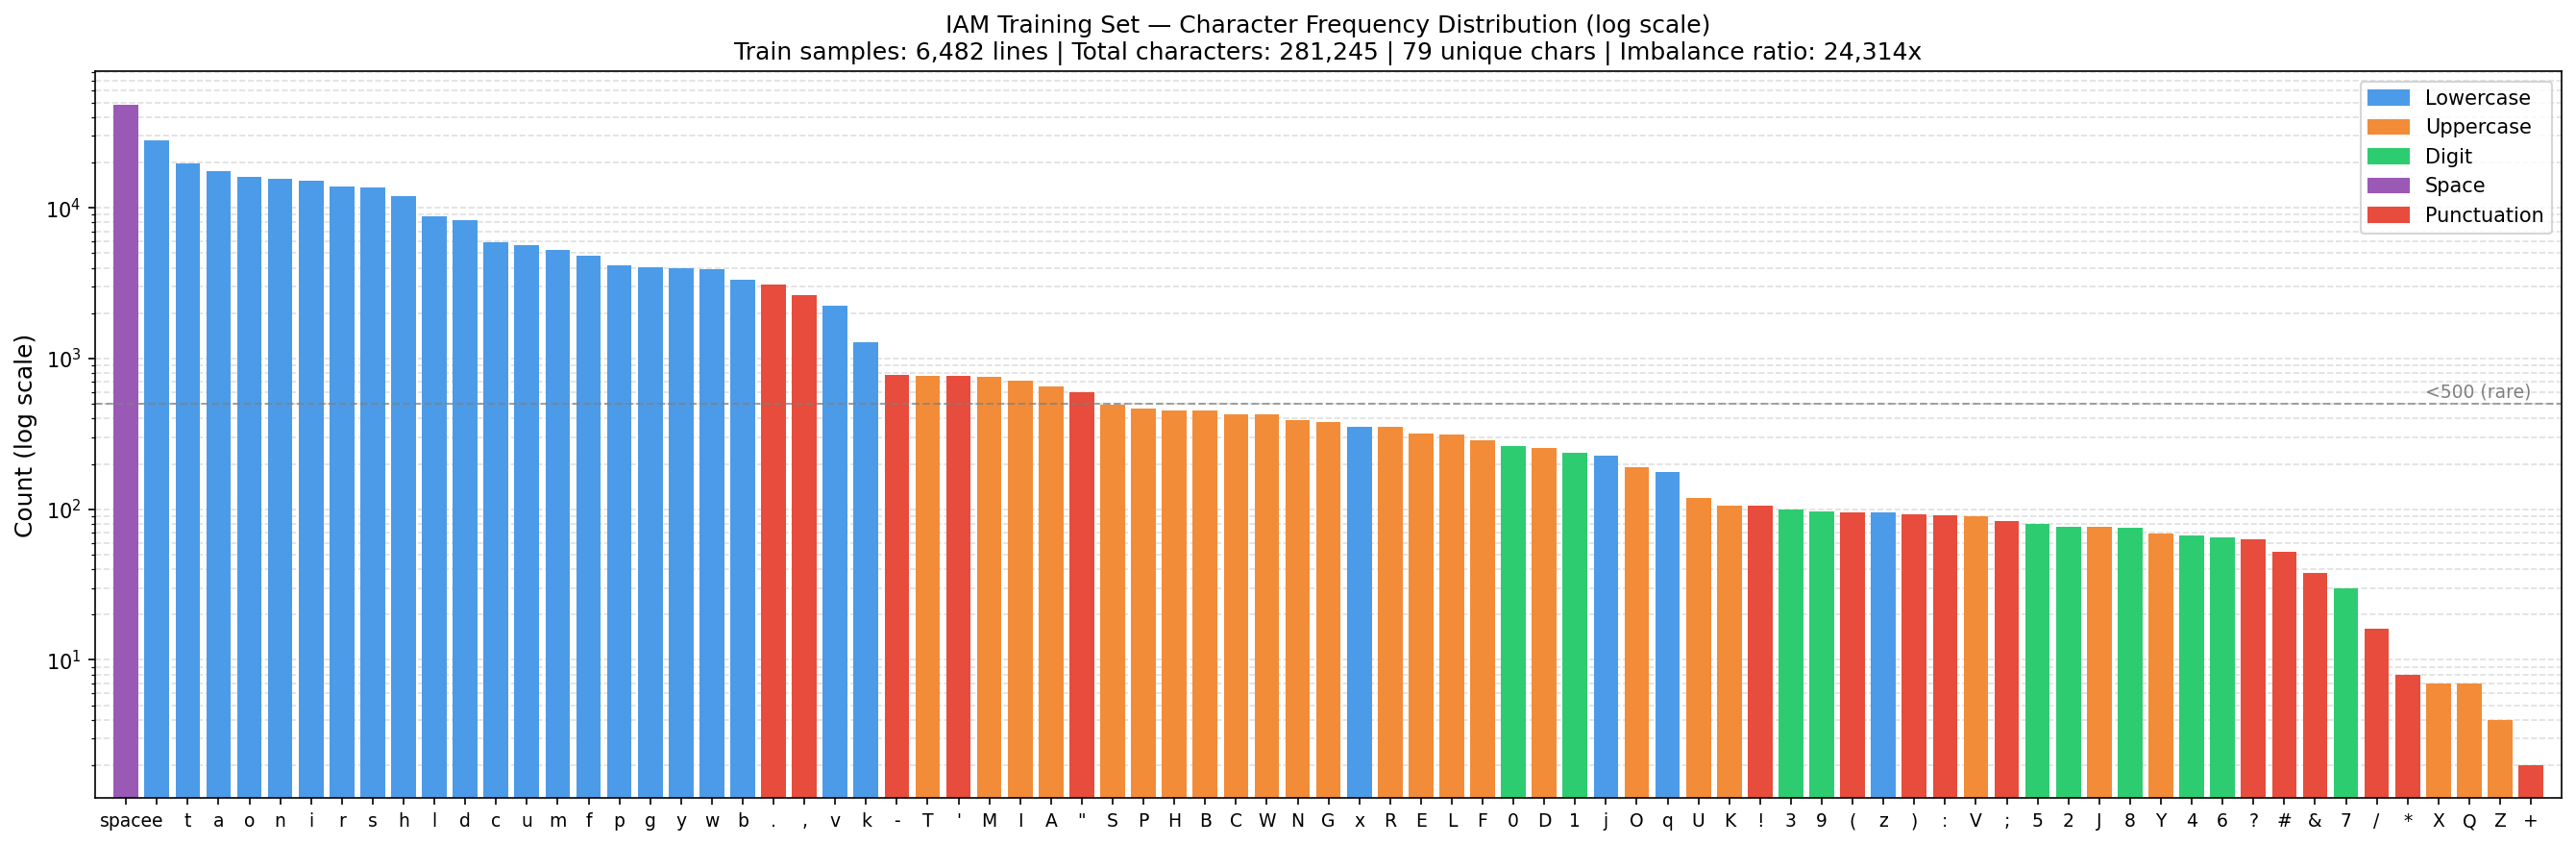
\includegraphics[width=\columnwidth]{char_freq_distribution.png}
  \caption{IAM training set character frequency distribution. The heavy skew motivates our targeted synthetic data pipeline; rare punctuation and uppercase letters are precisely the characters most likely to appear in student work.}
  \label{fig:charfreq}
\end{figure}

\subsection{VLM Annotation Quality Audit (V1 --- Aggressive)}

We audited all 10,373 IAM samples using Doubao Seed 2.0 Pro with a prompt instructing the model to ``err on the side of flagging'' any possible annotation error. Table~\ref{tab:v1audit} shows results: 34.3\% of samples were flagged, a surprisingly high rate that---as we show in Section~\ref{sec:crossmatrix}---reflects genuine visual ambiguity rather than true annotation error.

\begin{table}[h]
\centering
\caption{V1 VLM Audit Results}
\label{tab:v1audit}
\begin{tabular}{@{}lccc@{}}
\toprule
\textbf{Split} & \textbf{Total} & \textbf{Flagged} & \textbf{Rate} \\
\midrule
Train      & 6,482  & 2,144 & 33.1\% \\
Validation & 976    & 360   & 36.9\% \\
Test       & 2,915  & 1,053 & 36.1\% \\
\midrule
\textbf{Total} & \textbf{10,373} & \textbf{3,557} & \textbf{34.3\%} \\
\bottomrule
\end{tabular}
\end{table}

\subsection{VLM Annotation Quality Audit (V2 --- Conservative)}

A redesigned V2 prompt explicitly instructs the model to ``default to CORRECT'' and lists false-positive traps (digit 0 vs.\ letter O, British spelling, abbreviations, etc.). Applied to training only, V2 reduces the flag rate from 33.1\% to 12.6\%, removing 814 samples instead of 2,144. The contrast between V1 and V2 outcomes is itself a key finding (Section~\ref{sec:cleaning}).

\subsection{VLM Character Confusion Analysis}

Substitutions were extracted by character-level alignment (\texttt{difflib.SequenceMatcher}) between IAM ground-truth and VLM V1-corrected text, identifying \textbf{936 unique confusion pairs} totaling \textbf{5,058 substitution events}. Table~\ref{tab:confusion_top} shows the top 10 pairs. The dominant pattern is lowercase--lowercase confusion ($\approx$93\% of events), concentrated on visually similar cursive strokes: \texttt{o}$\leftrightarrow$\texttt{a} (271 combined), \texttt{n}$\leftrightarrow$\texttt{m} (135+), \texttt{r}$\leftrightarrow$\texttt{s} (192 combined).

These are \emph{exactly} the character pairs that are also hardest for a trained HTR model---a non-obvious finding with direct educational implications: the VLM's confusion table can serve as a cold-start confusion prior for the configurable corrector (Section~\ref{sec:corrector}).

\begin{table}[h]
\centering
\caption{Top-10 VLM Annotation Confusion Pairs. These pairs recur as the top model prediction errors (see Table~\ref{tab:crossmatrix}).}
\label{tab:confusion_top}
\begin{tabular}{@{}clcc@{}}
\toprule
\textbf{Rank} & \textbf{Pair} & \textbf{Count} & \textbf{Category} \\
\midrule
1  & \texttt{o}$\to$\texttt{a} & 155 & lower--lower \\
2  & \texttt{n}$\to$\texttt{m} & 135 & lower--lower \\
3  & \texttt{r}$\to$\texttt{s} & 133 & lower--lower \\
4  & \texttt{a}$\to$\texttt{o} & 116 & lower--lower \\
5  & \texttt{a}$\to$\texttt{e} & 109 & lower--lower \\
6  & \texttt{n}$\to$\texttt{u} & 96  & lower--lower \\
7  & \texttt{o}$\to$\texttt{e} & 76  & lower--lower \\
8  & \texttt{t}$\to$\texttt{h} & 75  & lower--lower \\
9  & \texttt{t}$\to$\texttt{d} & 68  & lower--lower \\
10 & \texttt{h}$\to$\texttt{l} & 60  & lower--lower \\
\bottomrule
\end{tabular}
\end{table}

Figure~\ref{fig:vlmconfusion} visualizes the top-35 VLM annotation confusion pairs.

\begin{figure}[t]
  \centering
  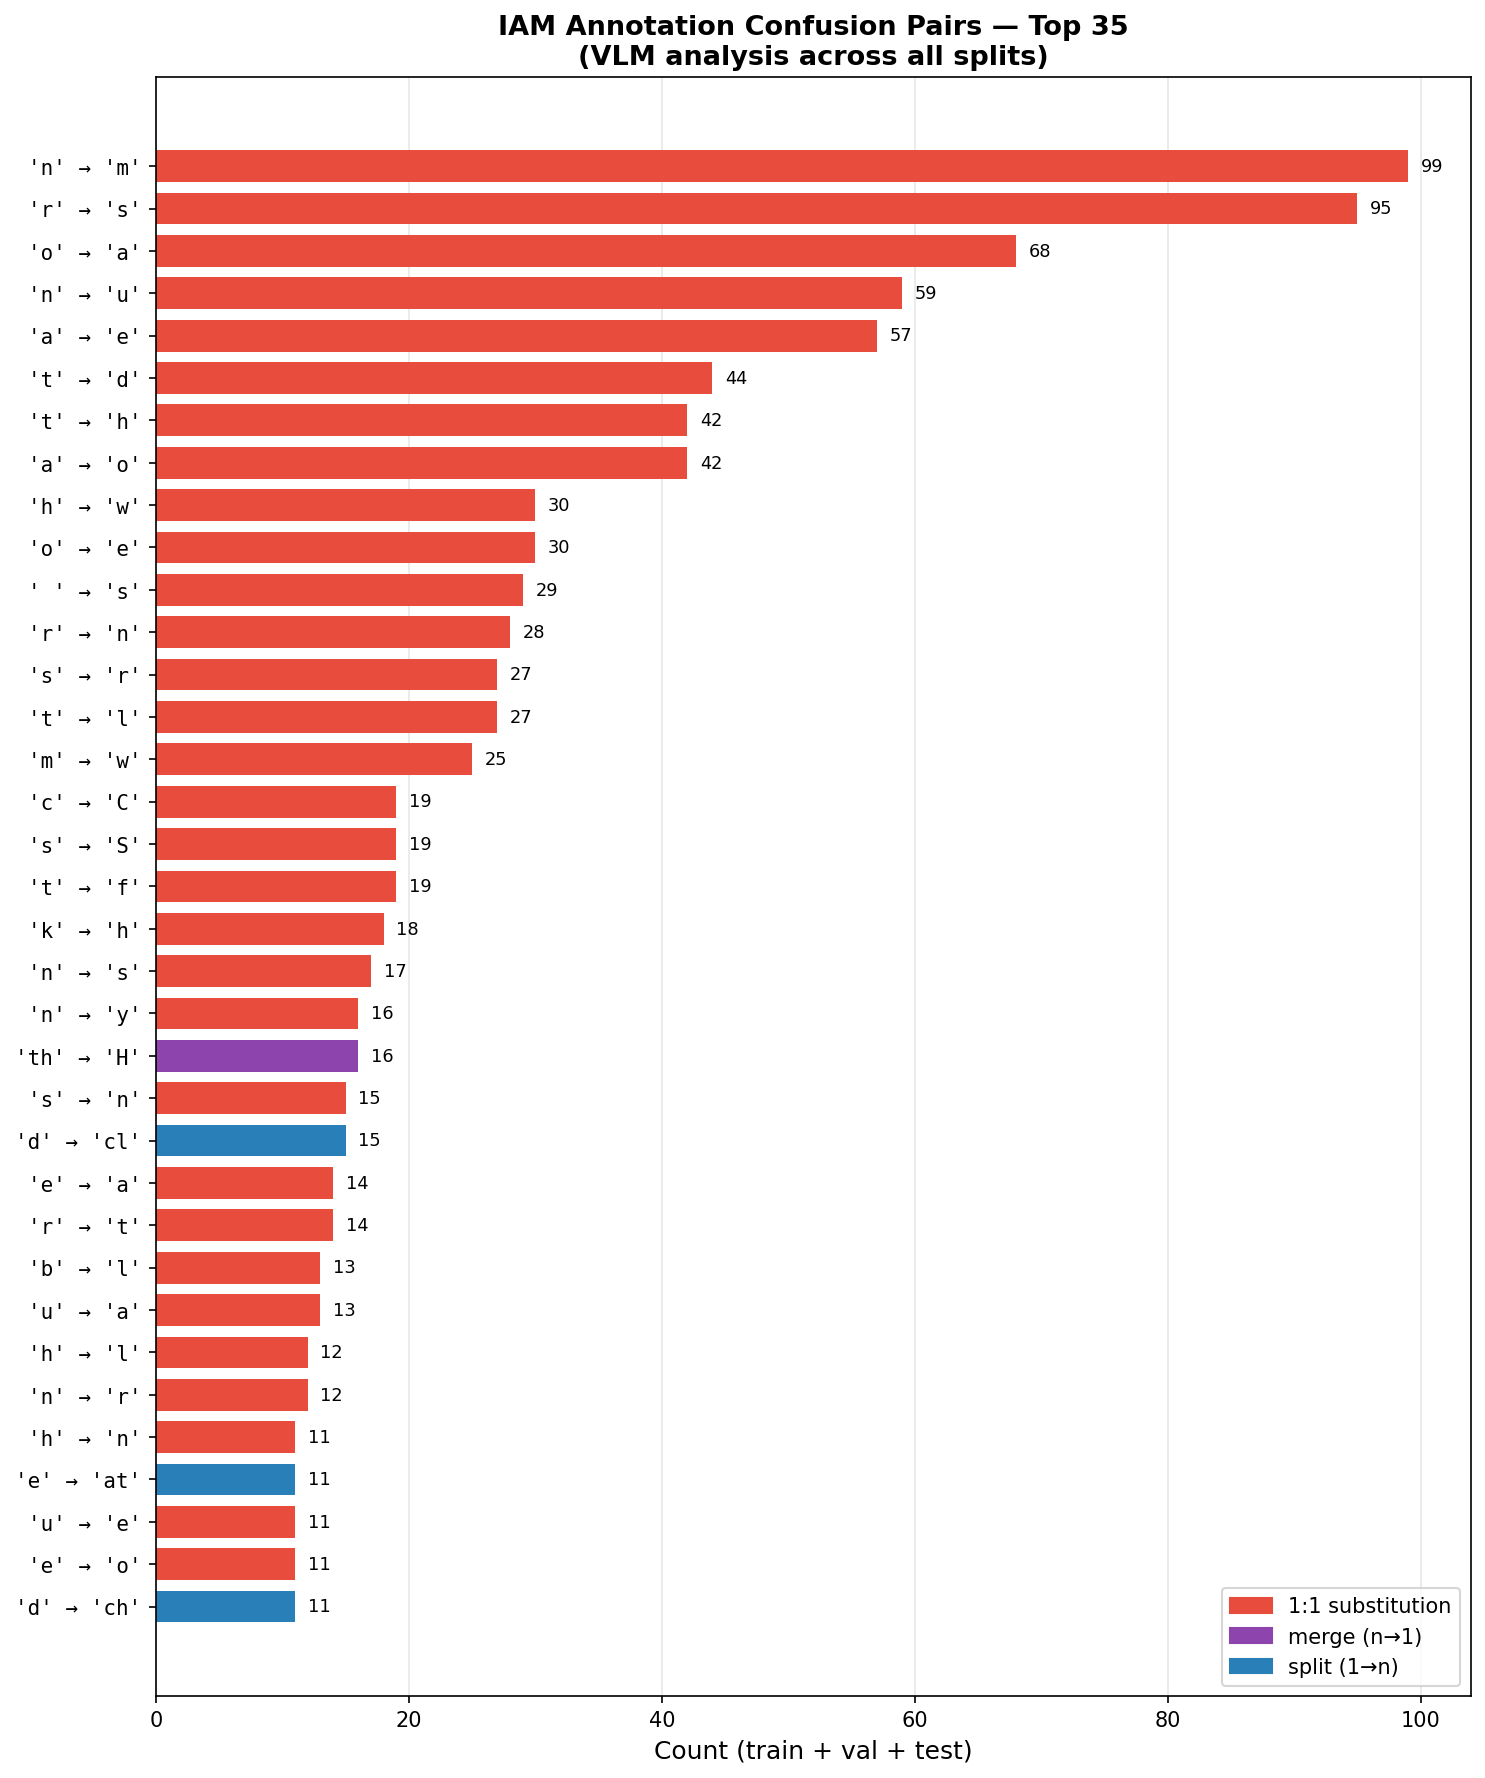
\includegraphics[width=\columnwidth]{vlm_confusion_top35.png}
  \caption{Top-35 VLM annotation confusion pairs (substitution count). Lowercase--lowercase pairs dominate; these form the default confusion prior available to teachers before any model training.}
  \label{fig:vlmconfusion}
\end{figure}

%% ============================================================
\section{Model Architecture}
%% ============================================================

\subsection{CRNN-CTC}

Our model follows the standard CRNN pipeline: CNN feature extractor $\to$ BiGRU encoder $\to$ CTC decoder. We adapt the VGG CRNN backbone (designed for $H=32$) to $H=64$ by modifying the final convolutional kernel to $(4,1)$, validated to outperform the original $(2,1)$ design at $H=64$ (7.35\% vs.\ 7.45\% val CER). The sequence encoder is a 2-layer Bidirectional GRU (hidden size=512), followed by a Linear$(1024\!\to\!80)$ projection with log-softmax. Total parameters: $\approx$16.7M. The model is intentionally compact: deployment in schools requires running on standard hardware without specialized GPU clusters.

\subsection{Training Details}

\begin{table}[h]
\centering
\caption{Training Hyperparameters (optimal configuration from Section~\ref{sec:hparam})}
\label{tab:hparams}
\begin{tabular}{@{}ll@{}}
\toprule
\textbf{Hyperparameter} & \textbf{Value} \\
\midrule
Optimizer       & AdamW, weight\_decay=$10^{-4}$ \\
Initial LR      & $3\times10^{-4}$ \\
LR Schedule     & ReduceLROnPlateau (patience=10) \\
Warmup          & 1 epoch linear \\
Batch size      & 64 \\
Gradient clip   & L2 norm $\leq 10.0$ \\
Dropout         & 0.1 (before BiGRU) \\
Epochs          & 150 (main) / 50 (search proxy) \\
Input height    & $H=64$, width variable \\
\bottomrule
\end{tabular}
\end{table}

%% ============================================================
\section{Synthetic Data Pipeline}
%% ============================================================

\subsection{Motivation}

The IAM character distribution is heavily skewed: rare characters such as \texttt{\#}, \texttt{*}, \texttt{;} appear fewer than 60 times in training. In educational settings these rare characters matter---students write equations, dates, and punctuated sentences. Font-based synthesis efficiently increases rare-character coverage.

\subsection{Text Sources}

We use a three-layer text pool: (1) IAM training labels ($\times2$, $\sim$13,000 sentences) for in-distribution vocabulary; (2) LLM-generated rare-character sentences ($\sim$12,000), prompted from Doubao Seed 2.0 Pro to ensure each target character appears at least twice per sentence; and (3) rule-based template sentences ($\sim$3,000) with random slots for digits, dates, and punctuation. Combined pool: $\sim$28,000 sentences.

\subsection{Rendering}

Font rendering uses trdg~\cite{belval2019} with 14 fonts (9 handwriting-style, 5 print). Each image: $H=64$px, random skew (0--3$^\circ$), random blur (0--1px), random distortion. We generate a single 65,000-sample LMDB; training experiments use fixed-seed subsets for comparability. Figure~\ref{fig:synth} shows representative synthetic samples; Figure~\ref{fig:synthfreq} confirms balanced rare-character coverage.

\begin{figure}[t]
  \centering
  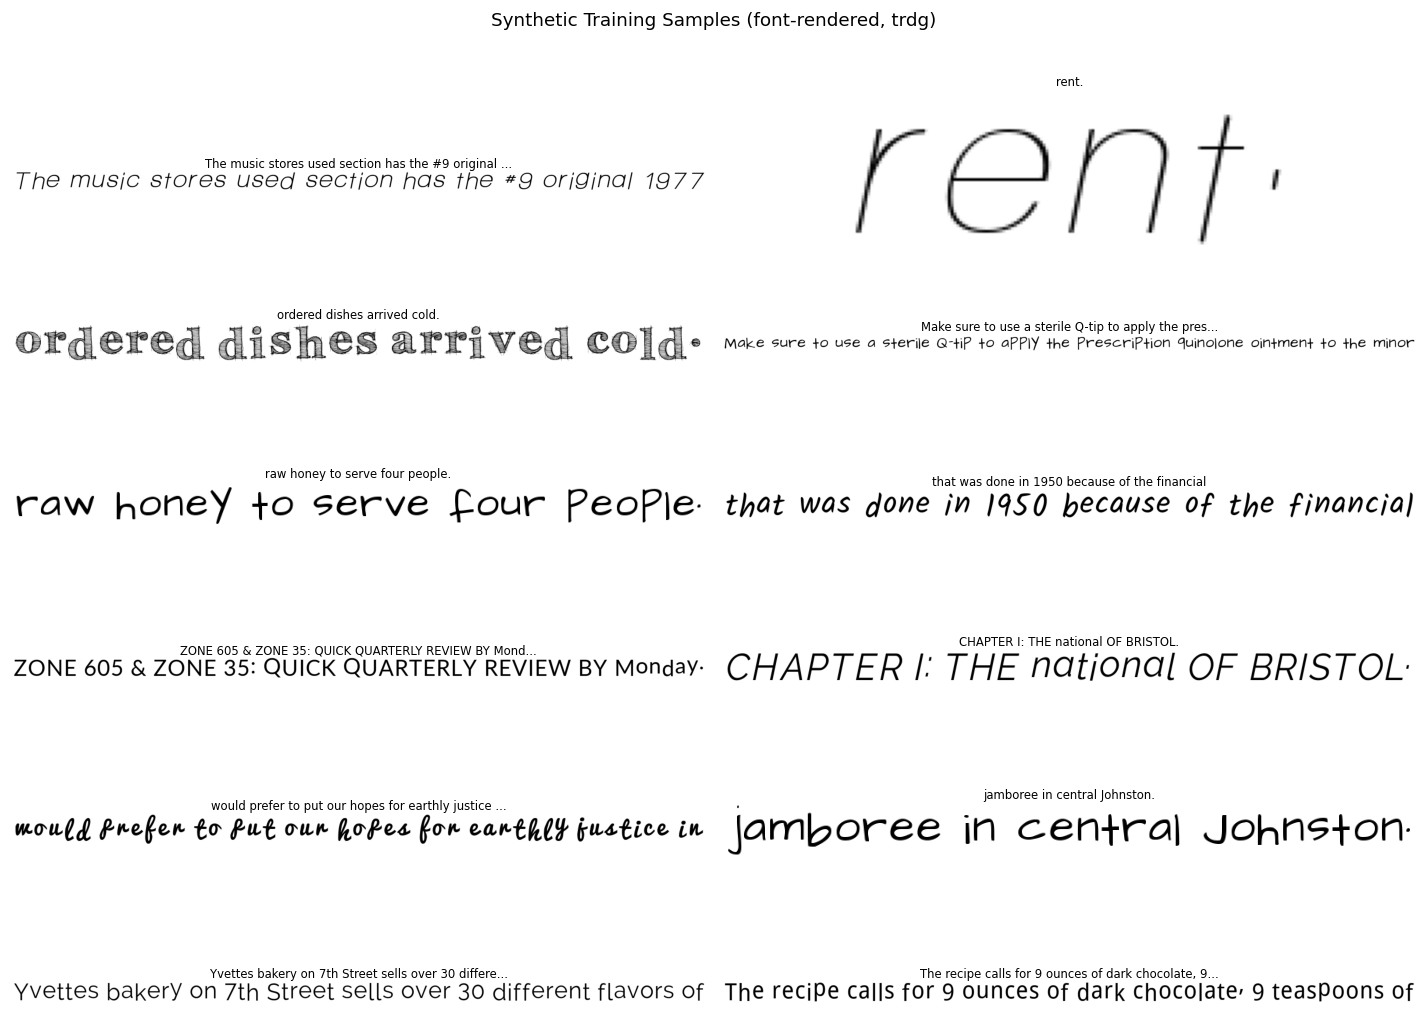
\includegraphics[width=\columnwidth]{synth_samples.png}
  \caption{Representative synthetic training samples. Nine handwriting-style and five print fonts are used with random augmentation to simulate within-class variation.}
  \label{fig:synth}
\end{figure}

\begin{figure}[t]
  \centering
  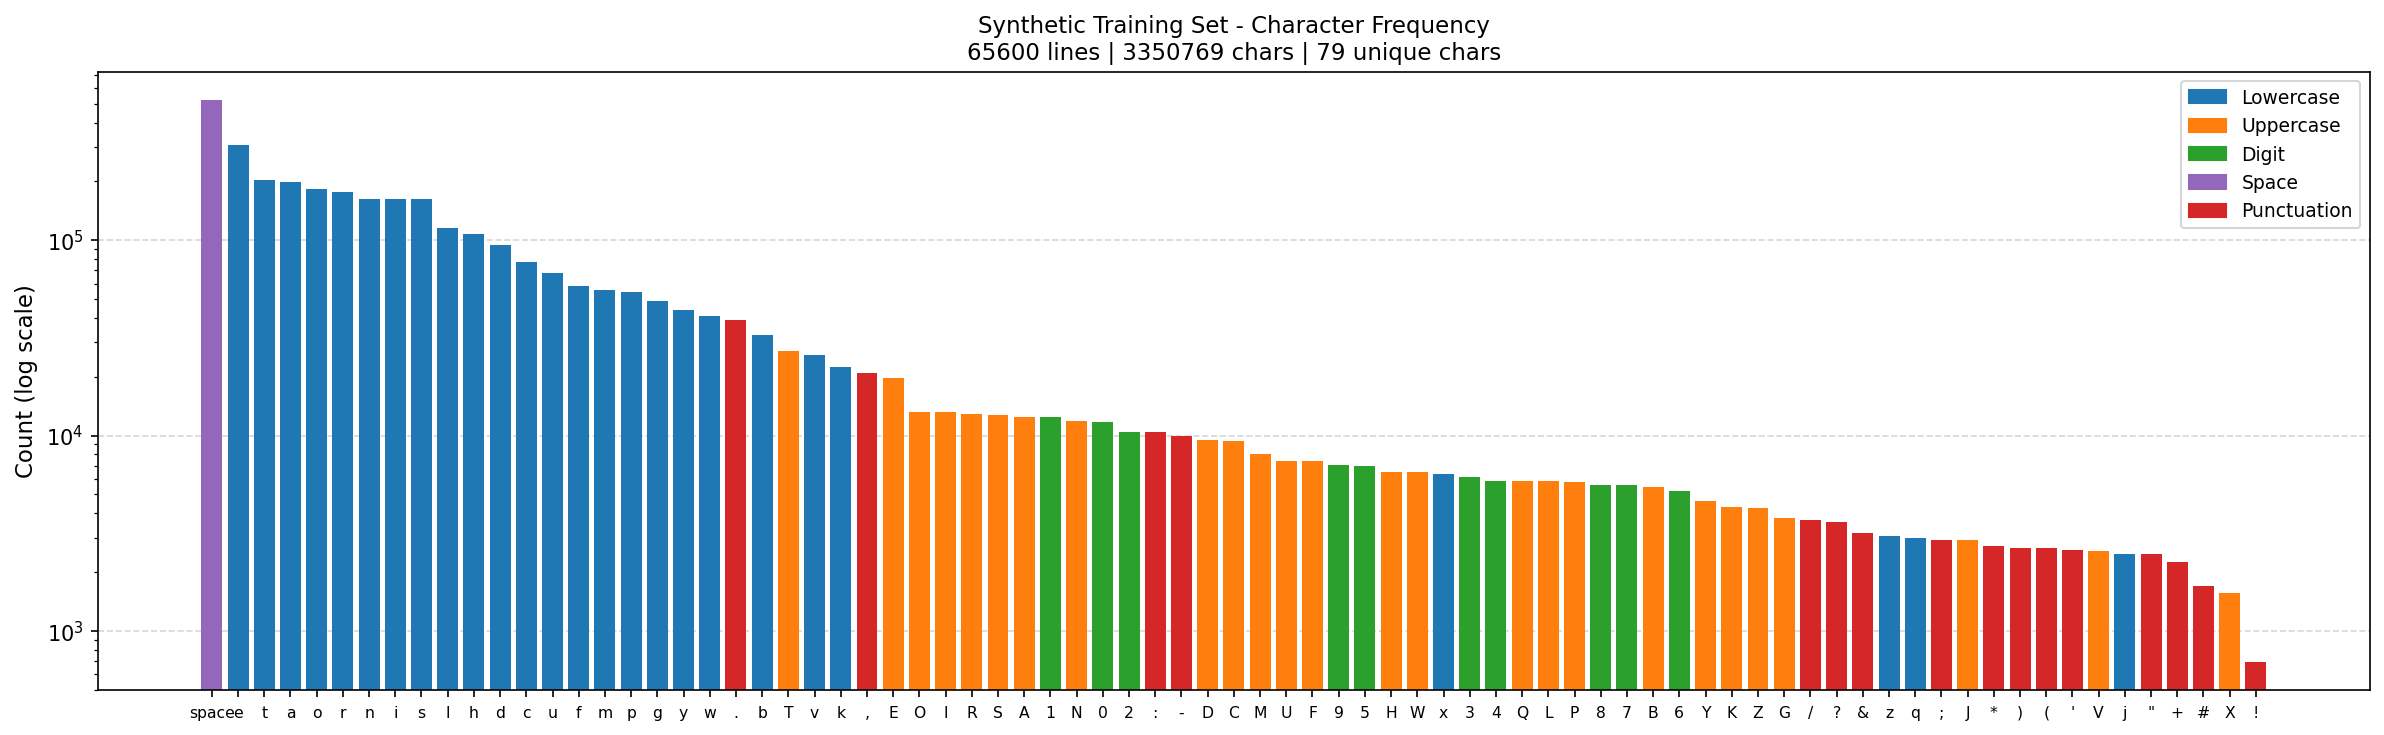
\includegraphics[width=\columnwidth]{synth_char_freq.png}
  \caption{Character frequency in the synthetic pool (65,000 samples). Rare characters (\texttt{\#}, \texttt{;}, \texttt{:}, uppercase) are explicitly oversampled via LLM-generated text, addressing the IAM class imbalance in Fig.~\ref{fig:charfreq}.}
  \label{fig:synthfreq}
\end{figure}

%% ============================================================
\section{Hyperparameter Search}
\label{sec:hparam}
%% ============================================================

\subsection{Protocol}

Greedy sequential search: change one hyperparameter at a time, keep if validation CER improves $>0.05\%$ relative. All runs use 50 epochs as a proxy budget. Seven GPUs run in parallel.

\subsection{Results}

Table~\ref{tab:hparam_search} summarizes all 14 runs. Figure~\ref{fig:hparam} visualizes the val CER across configurations.

\begin{figure}[t]
  \centering
  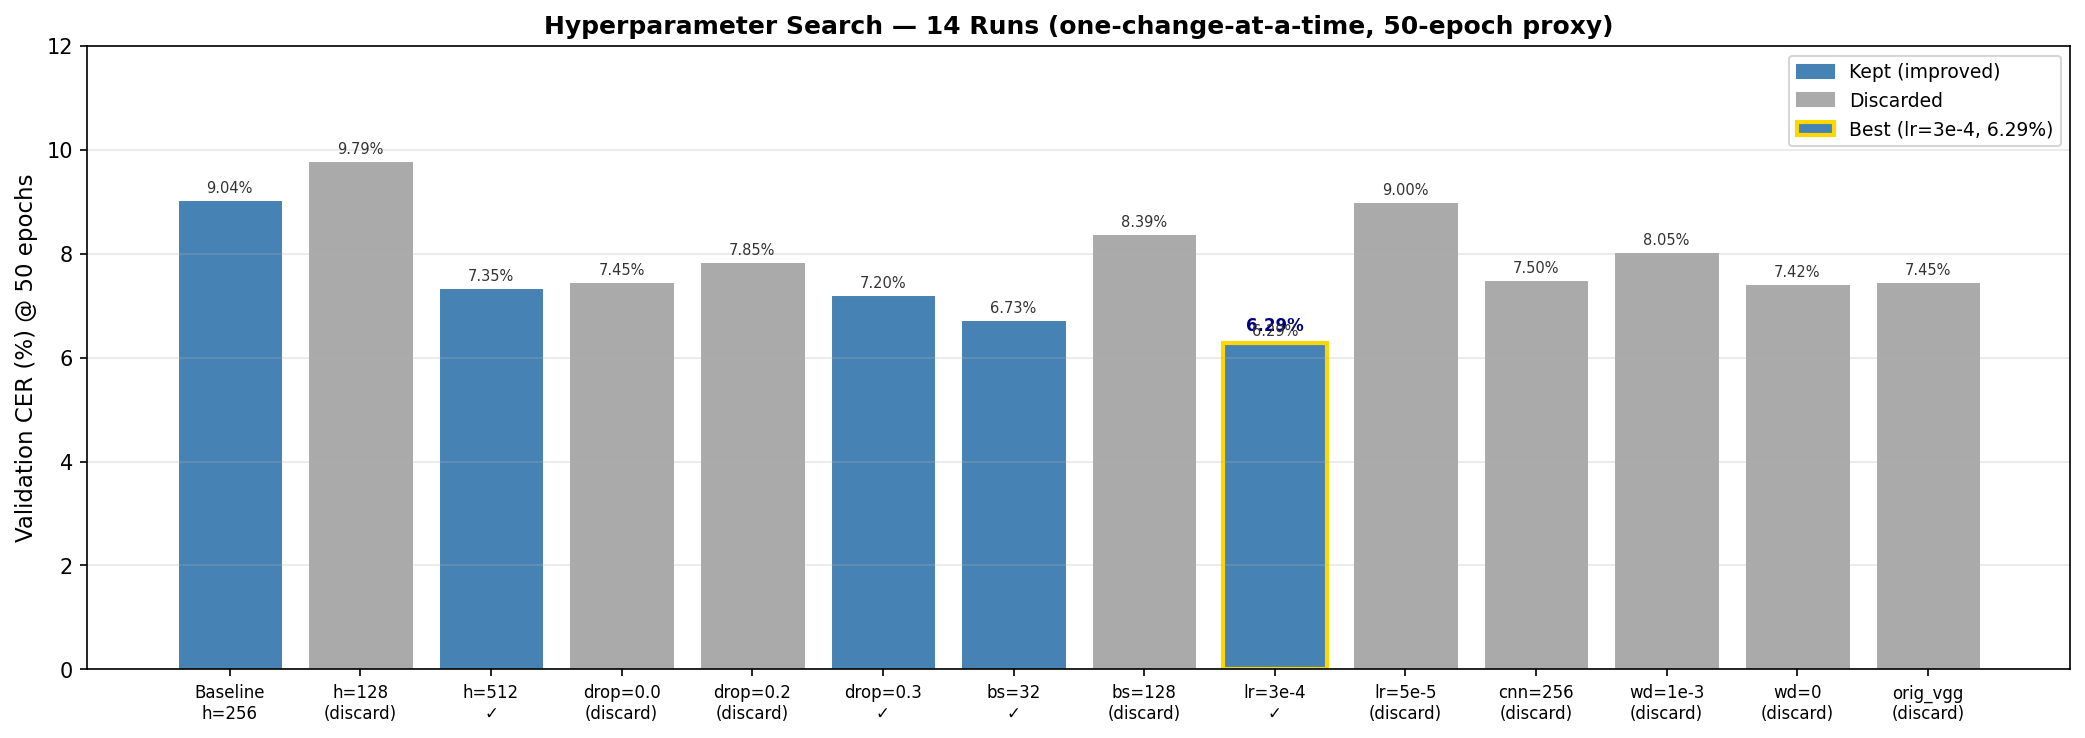
\includegraphics[width=\columnwidth]{hparam_search_chart.png}
  \caption{Hyperparameter search results across 14 configurations. Hidden size 512 and lr=$3\times10^{-4}$ provide the two largest individual gains.}
  \label{fig:hparam}
\end{figure}

\begin{table}[h]
\centering
\caption{Hyperparameter Search Results (50-epoch proxy)}
\label{tab:hparam_search}
\begin{tabular}{@{}clccc@{}}
\toprule
\textbf{Run} & \textbf{Change} & \textbf{Val CER} & $\boldsymbol{\Delta}$ & \textbf{Decision} \\
\midrule
00 & Baseline (hidden=256)    & 9.04\% & ---     & Keep \\
01 & hidden=128               & 9.79\% & +0.75\% & Discard \\
\textbf{02} & \textbf{hidden=512} & \textbf{7.35\%} & \textbf{$-$1.69\%} & \textbf{Keep} \\
03 & dropout=0.0              & 7.45\% & +0.10\% & Discard \\
04 & dropout=0.2              & 7.85\% & +0.50\% & Discard \\
05 & dropout=0.3              & 7.20\% & $-$0.15\% & Keep \\
06 & batch\_size=32           & 6.73\% & $-$0.62\% & Keep \\
07 & batch\_size=128          & 8.39\% & +1.04\% & Discard \\
\textbf{08} & \textbf{lr=$3\times10^{-4}$} & \textbf{6.29\%} & \textbf{$-$1.06\%} & \textbf{Keep} \\
09 & lr=$5\times10^{-5}$      & 9.00\% & +2.71\% & Discard \\
10 & cnn\_out=256             & 7.50\% & +1.21\% & Discard \\
11 & weight\_decay=$10^{-3}$  & 8.05\% & +1.76\% & Discard \\
12 & weight\_decay=0          & 7.42\% & +1.13\% & Discard \\
13 & Original VGG kernel      & 7.45\% & +1.16\% & Discard \\
\bottomrule
\end{tabular}
\end{table}

\texttt{hidden=512} produced the largest single improvement ($9.04\%\to7.35\%$), indicating the BiGRU was the primary bottleneck. \texttt{lr=$3\times10^{-4}$} provided the second-largest gain ($7.35\%\to6.29\%$), reflecting faster convergence within the 50-epoch proxy budget.

%% ============================================================
\section{Experiments: Training Data Choices}
%% ============================================================

\subsection{Experimental Setup}

All main experiments use the optimal configuration from Section~\ref{sec:hparam}, trained for 150 epochs. Table~\ref{tab:exp_index} defines the five experiment series. \textbf{Evaluation metric:} Character Error Rate (CER) $= \frac{\text{edit\_distance}(\hat{y}, y)}{\max(|y|, 1)} \times 100\%$.

\begin{table}[h]
\centering
\caption{Experiment Series Index}
\label{tab:exp_index}
\begin{tabular}{@{}lll@{}}
\toprule
\textbf{Series} & \textbf{Base Training Set} & \textbf{Note} \\
\midrule
Exp1      & Full IAM (6,482)    & No synth; optimal hparams \\
Exp2      & V1-cleaned (4,338)  & Aggressive VLM cleaning; no synth \\
Exp3-$N$x & Full IAM + $N\times$ synth & $N \in \{1,2,3,5,7,10\}$ \\
Exp4-$N$x & V1-cleaned + $N\times$ synth & $N \in \{1,2,3,5,7,10\}$ \\
Exp5-$N$x & V2-cleaned (5,668) + $N\times$ synth & $N \in \{0,1,2,3,5,7,10\}$ \\
\bottomrule
\end{tabular}
\end{table}

\textbf{Exp1} establishes the post-hparam-search baseline on the full IAM set. \textbf{Exp2} isolates the effect of aggressive VLM cleaning (V1 prompt, $-$33\% of data). \textbf{Exp3} ($N\!\in\!\{1,2,3,5,7,10\}$) tests synthetic augmentation at scale on the full set. \textbf{Exp4} ($N\!\in\!\{1,2,3,5,7,10\}$) probes the interaction between data removal and augmentation under a reduced real-data anchor. \textbf{Exp5} ($N\!\in\!\{0,1,2,3,5,7,10\}$) repeats the augmentation study with the more conservative V2-cleaned set.

\subsection{Effect of VLM Annotation Cleaning}
\label{sec:cleaning}

\begin{table}[h]
\centering
\caption{Full vs.\ VLM-Cleaned IAM Results}
\label{tab:cleaning}
\begin{tabular}{@{}llcc@{}}
\toprule
\textbf{Exp} & \textbf{Training Set} & \textbf{Samples} & \textbf{Test CER} \\
\midrule
Exp1          & Full IAM       & 6,482 & 8.43\% \\
Exp2          & V1 cleaned     & 4,338 & 10.33\% $\uparrow$ \\
Exp5-base     & V2 cleaned     & 5,668 & 8.36\% $\approx$ \\
\bottomrule
\end{tabular}
\end{table}

Aggressive V1 cleaning ($-$33\% of data) significantly degrades test CER from 8.43\% to 10.33\%. Conservative V2 cleaning ($-$12.6\%) is neutral ($8.43\%\to8.36\%$). This result is explained by the cross-matrix finding in Section~\ref{sec:crossmatrix}: the samples the VLM flags are concentrated in visually ambiguous character regions where both annotators and the model struggle. Removing them does not clean noise---it removes informative, hard training examples.

\subsection{Synthetic Data Augmentation}

\begin{table}[h]
\centering
\caption{Synthetic Augmentation Results: All Three Series}
\label{tab:synth}
\begin{tabular}{@{}llcc@{}}
\toprule
\textbf{Exp} & \textbf{Base Set} & \textbf{Scale} & \textbf{Test CER} \\
\midrule
\multicolumn{4}{@{}l}{\textit{Exp3 --- Full IAM + synthetic (6,482 base samples)}} \\
Exp1          & Full IAM   & 0$\times$  & 8.43\% \\
Exp3-1x       & Full IAM   & 1$\times$  & 7.93\% \\
Exp3-2x       & Full IAM   & 2$\times$  & 7.88\% \\
Exp3-3x       & Full IAM   & 3$\times$  & 7.66\% \\
Exp3-5x       & Full IAM   & 5$\times$  & 7.63\% \\
Exp3-7x       & Full IAM   & 7$\times$  & 7.75\% \\
\textbf{Exp3-10x} & \textbf{Full IAM} & \textbf{10$\times$} & \textbf{7.52\%} \\
\midrule
\multicolumn{4}{@{}l}{\textit{Exp4 --- V1-cleaned IAM + synthetic (4,338 base samples)}} \\
Exp2          & V1 cleaned & 0$\times$  & 10.33\% \\
Exp4-1x       & V1 cleaned & 1$\times$  & 8.94\% \\
Exp4-2x       & V1 cleaned & 2$\times$  & 8.76\% \\
\textbf{Exp4-3x} & \textbf{V1 cleaned} & \textbf{3$\times$} & \textbf{8.61\%} \\
Exp4-5x       & V1 cleaned & 5$\times$  & 8.86\% $\uparrow$ \\
Exp4-7x       & V1 cleaned & 7$\times$  & 8.91\% $\uparrow$ \\
Exp4-10x      & V1 cleaned & 10$\times$ & 9.07\% $\uparrow$ \\
\midrule
\multicolumn{4}{@{}l}{\textit{Exp5 --- V2-cleaned IAM + synthetic (5,668 base samples)}} \\
Exp5-base     & V2 cleaned & 0$\times$  & 8.38\% \\
Exp5-1x       & V2 cleaned & 1$\times$  & 8.09\% \\
Exp5-2x       & V2 cleaned & 2$\times$  & 7.99\% \\
Exp5-3x       & V2 cleaned & 3$\times$  & 8.03\% \\
Exp5-5x       & V2 cleaned & 5$\times$  & 7.92\% \\
Exp5-7x       & V2 cleaned & 7$\times$  & 8.17\% \\
Exp5-10x      & V2 cleaned & 10$\times$ & 8.06\% \\
\bottomrule
\end{tabular}
\end{table}

Synthetic augmentation provides consistent greedy CER improvement for Exp3 (full IAM base): CER decreases from 8.43\% to 7.52\% at $10\times$ scale, a 10.8\% relative improvement. Exp4 (V1-cleaned + synth) reveals an important finding for educational deployment: CER \emph{increases} beyond $3\times$ scale when the real-data anchor is reduced to 4,338 samples, ultimately worsening to 9.07\% at $10\times$. This ``anchor effect'' implies a \textbf{minimum real-data threshold} below which synthetic augmentation is counter-productive---a practical constraint for schools with limited annotated data. Exp5 shows that conservative cleaning (removing only 12.6\% of data) avoids the anchor effect and achieves $\sim$7.9\% CER, narrowing the gap to Exp3.

\subsection{Per-Character Error Analysis}

\begin{table}[h]
\centering
\caption{Per-Character CER: Exp1 vs.\ Exp3-10x (selected)}
\label{tab:perchar}
\begin{tabular}{@{}lcrrc@{}}
\toprule
\textbf{Char} & \textbf{Count} & \textbf{Exp1} & \textbf{Exp3-10x} & $\boldsymbol{\Delta}$ \\
\midrule
\texttt{\#} & 5   & 100.0\% & 60.0\%  & $-$40.0\% \\
\texttt{;}  & 60  & 41.7\%  & 21.7\%  & $-$20.0\% \\
\texttt{U}  & 11  & 36.4\%  & 18.2\%  & $-$18.2\% \\
\texttt{R}  & 67  & 35.8\%  & 20.9\%  & $-$14.9\% \\
\texttt{:}  & 29  & 55.2\%  & 41.4\%  & $-$13.8\% \\
\texttt{!}  & 47  & 38.3\%  & 25.5\%  & $-$12.8\% \\
\texttt{0}  & 34  & 38.2\%  & 26.5\%  & $-$11.8\% \\
\texttt{W}  & 122 & 32.0\%  & 20.5\%  & $-$11.5\% \\
\texttt{z}  & 45  & 35.6\%  & 40.0\%  & +4.4\%    \\
\bottomrule
\end{tabular}
\end{table}

The largest improvements concentrate on the rare characters targeted by our synthesis pipeline---exactly the characters appearing in student math and science work. The small regression on \texttt{z} is attributable to font rendering domain shift.

\subsection{VLM Confusion vs.\ Model Confusion: A Shared Ambiguity Structure}
\label{sec:crossmatrix}

The central hypothesis motivating our configurable corrector is that VLM annotation confusion and model prediction confusion share the same underlying structure---both reflecting physical visual ambiguity rather than system-specific biases. If this is true, VLM confusion tables derived without any model training can serve as cold-start confusion priors for educational deployment.

We extract all character pairs with count $\geq 5$ in \emph{both} the VLM confusion matrix (character-level alignment of IAM labels vs.\ VLM-corrected text) and the model confusion matrix (Levenshtein alignment of model outputs vs.\ ground truth on the test set). This yields \textbf{65 shared lowercase substitution pairs}. Spearman rank correlation:
\begin{equation}
  \rho = 0.636, \quad p < 0.0001 \quad (n = 65 \text{ pairs})
\end{equation}

\noindent We partition pairs into three groups based on cursive stroke properties:

\begin{itemize}
  \item \textbf{Round/oval} (\texttt{o,a,e,c,g,q}): characters formed from closed or nearly-closed oval strokes---the most visually ambiguous in cursive.
  \item \textbf{Stroke/ascender} (\texttt{n,m,u,r,s,h,l,t}): characters distinguished by stroke count, ascender height, or loop presence.
  \item \textbf{Other}: cross-category or less visually motivated pairs.
\end{itemize}

\begin{table}[h]
\centering
\caption{Per-Category Spearman Correlation (VLM vs.\ Model Confusion). The gradient reflects increasing visual distinctiveness across categories.}
\label{tab:crossmatrix}
\begin{tabular}{@{}lccc@{}}
\toprule
\textbf{Category} & \textbf{$n$} & \textbf{$\rho$} & \textbf{$p$} \\
\midrule
Round/oval (o,a,e,c,g,q)         & 10 & \textbf{0.942} & $<$0.001 \\
Stroke/ascender (n,m,u,r,s,h,l,t)& 23 & 0.651          & $<$0.001 \\
Other                              & 32 & 0.354          & 0.047    \\
\midrule
\textbf{Global}                    & \textbf{65} & \textbf{0.636} & $<$0.0001 \\
\bottomrule
\end{tabular}
\end{table}

\begin{figure}[t]
  \centering
  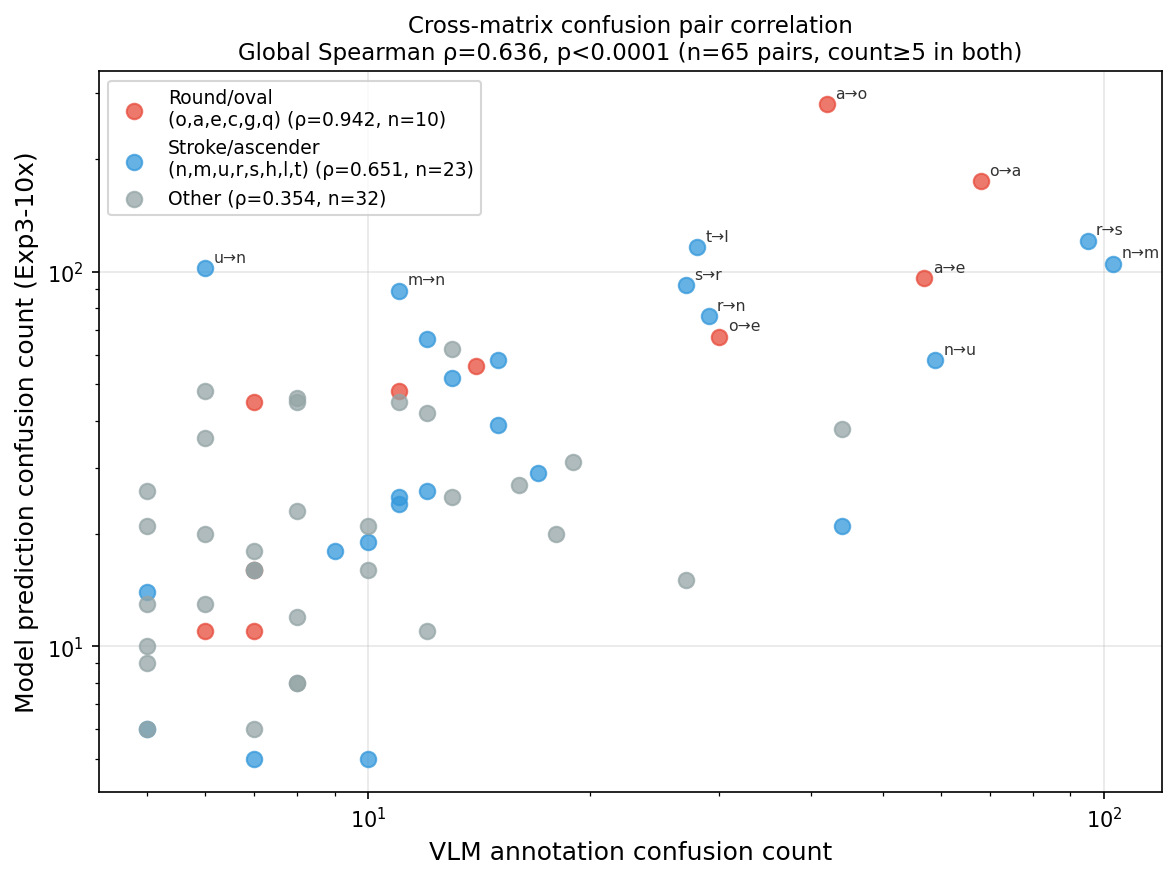
\includegraphics[width=\columnwidth]{cross_matrix_scatter.png}
  \caption{Log-log scatter of VLM confusion count vs.\ model confusion count for 65 shared pairs. Red: round/oval ($\rho=0.942$); blue: stroke/ascender ($\rho=0.651$); gray: other ($\rho=0.354$). The strong correlation within visually motivated categories confirms a shared physical cause---and validates VLM confusion as a cold-start prior.}
  \label{fig:crossscatter}
\end{figure}

\begin{figure}[t]
  \centering
  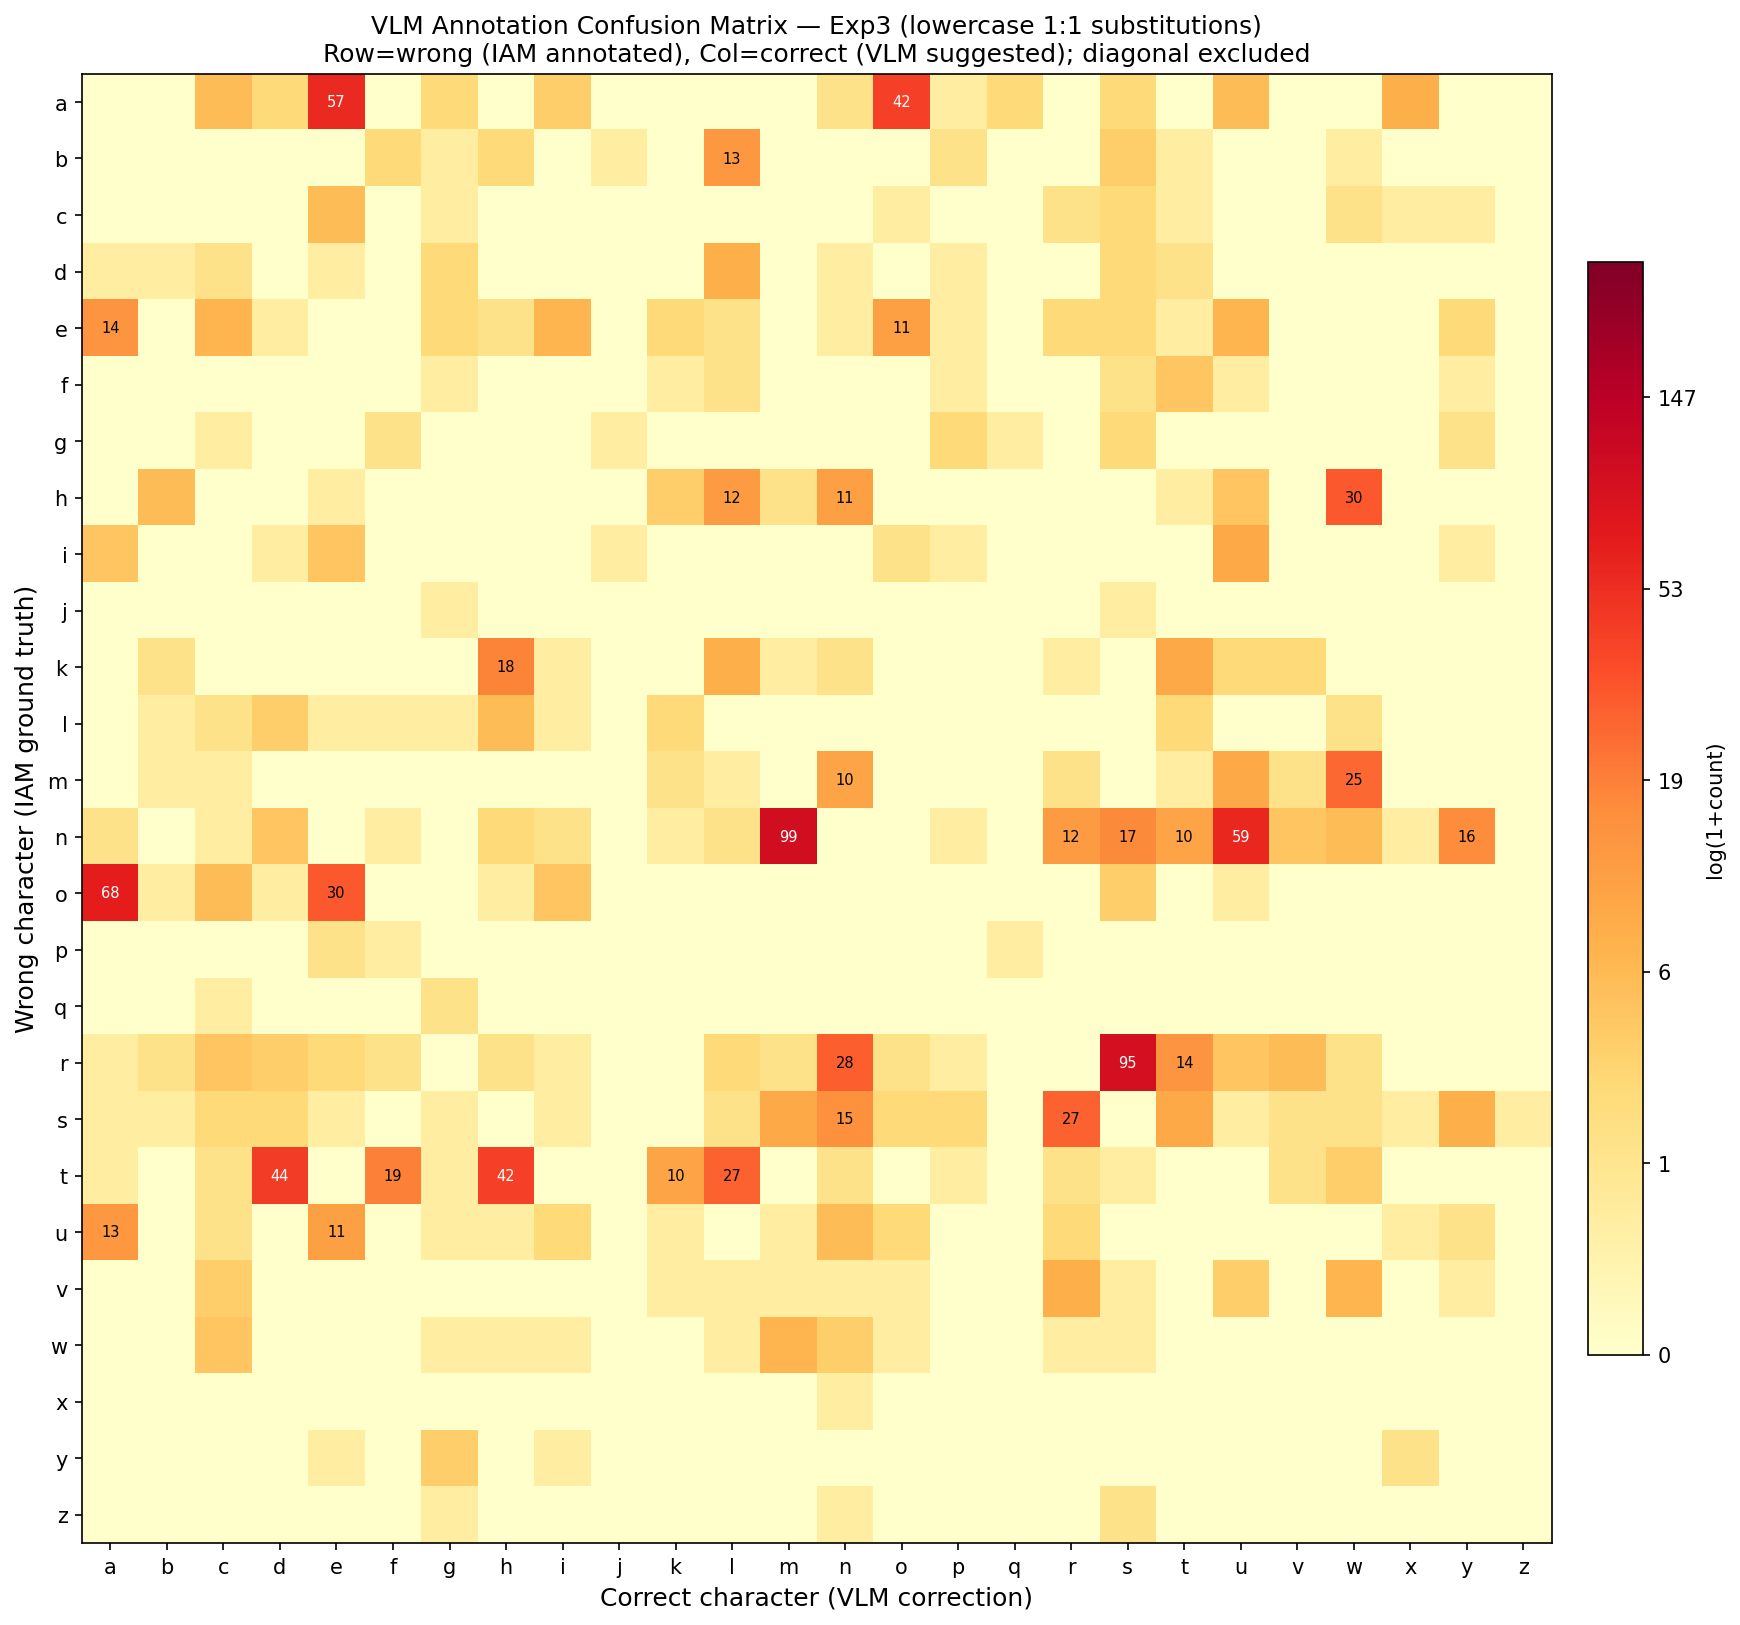
\includegraphics[width=\columnwidth]{vlm_confusion_matrix_1to1.png}
  \caption{VLM annotation confusion matrix (lowercase 1:1 substitutions). Row=IAM annotated, Col=VLM correction. Cell intensity is $\log(1{+}\text{count})$; same color scale as Figs.~\ref{fig:modelmatrix_exp3}--\ref{fig:modelmatrix_exp5}.}
  \label{fig:vlmmatrix}
\end{figure}

\begin{figure}[t]
  \centering
  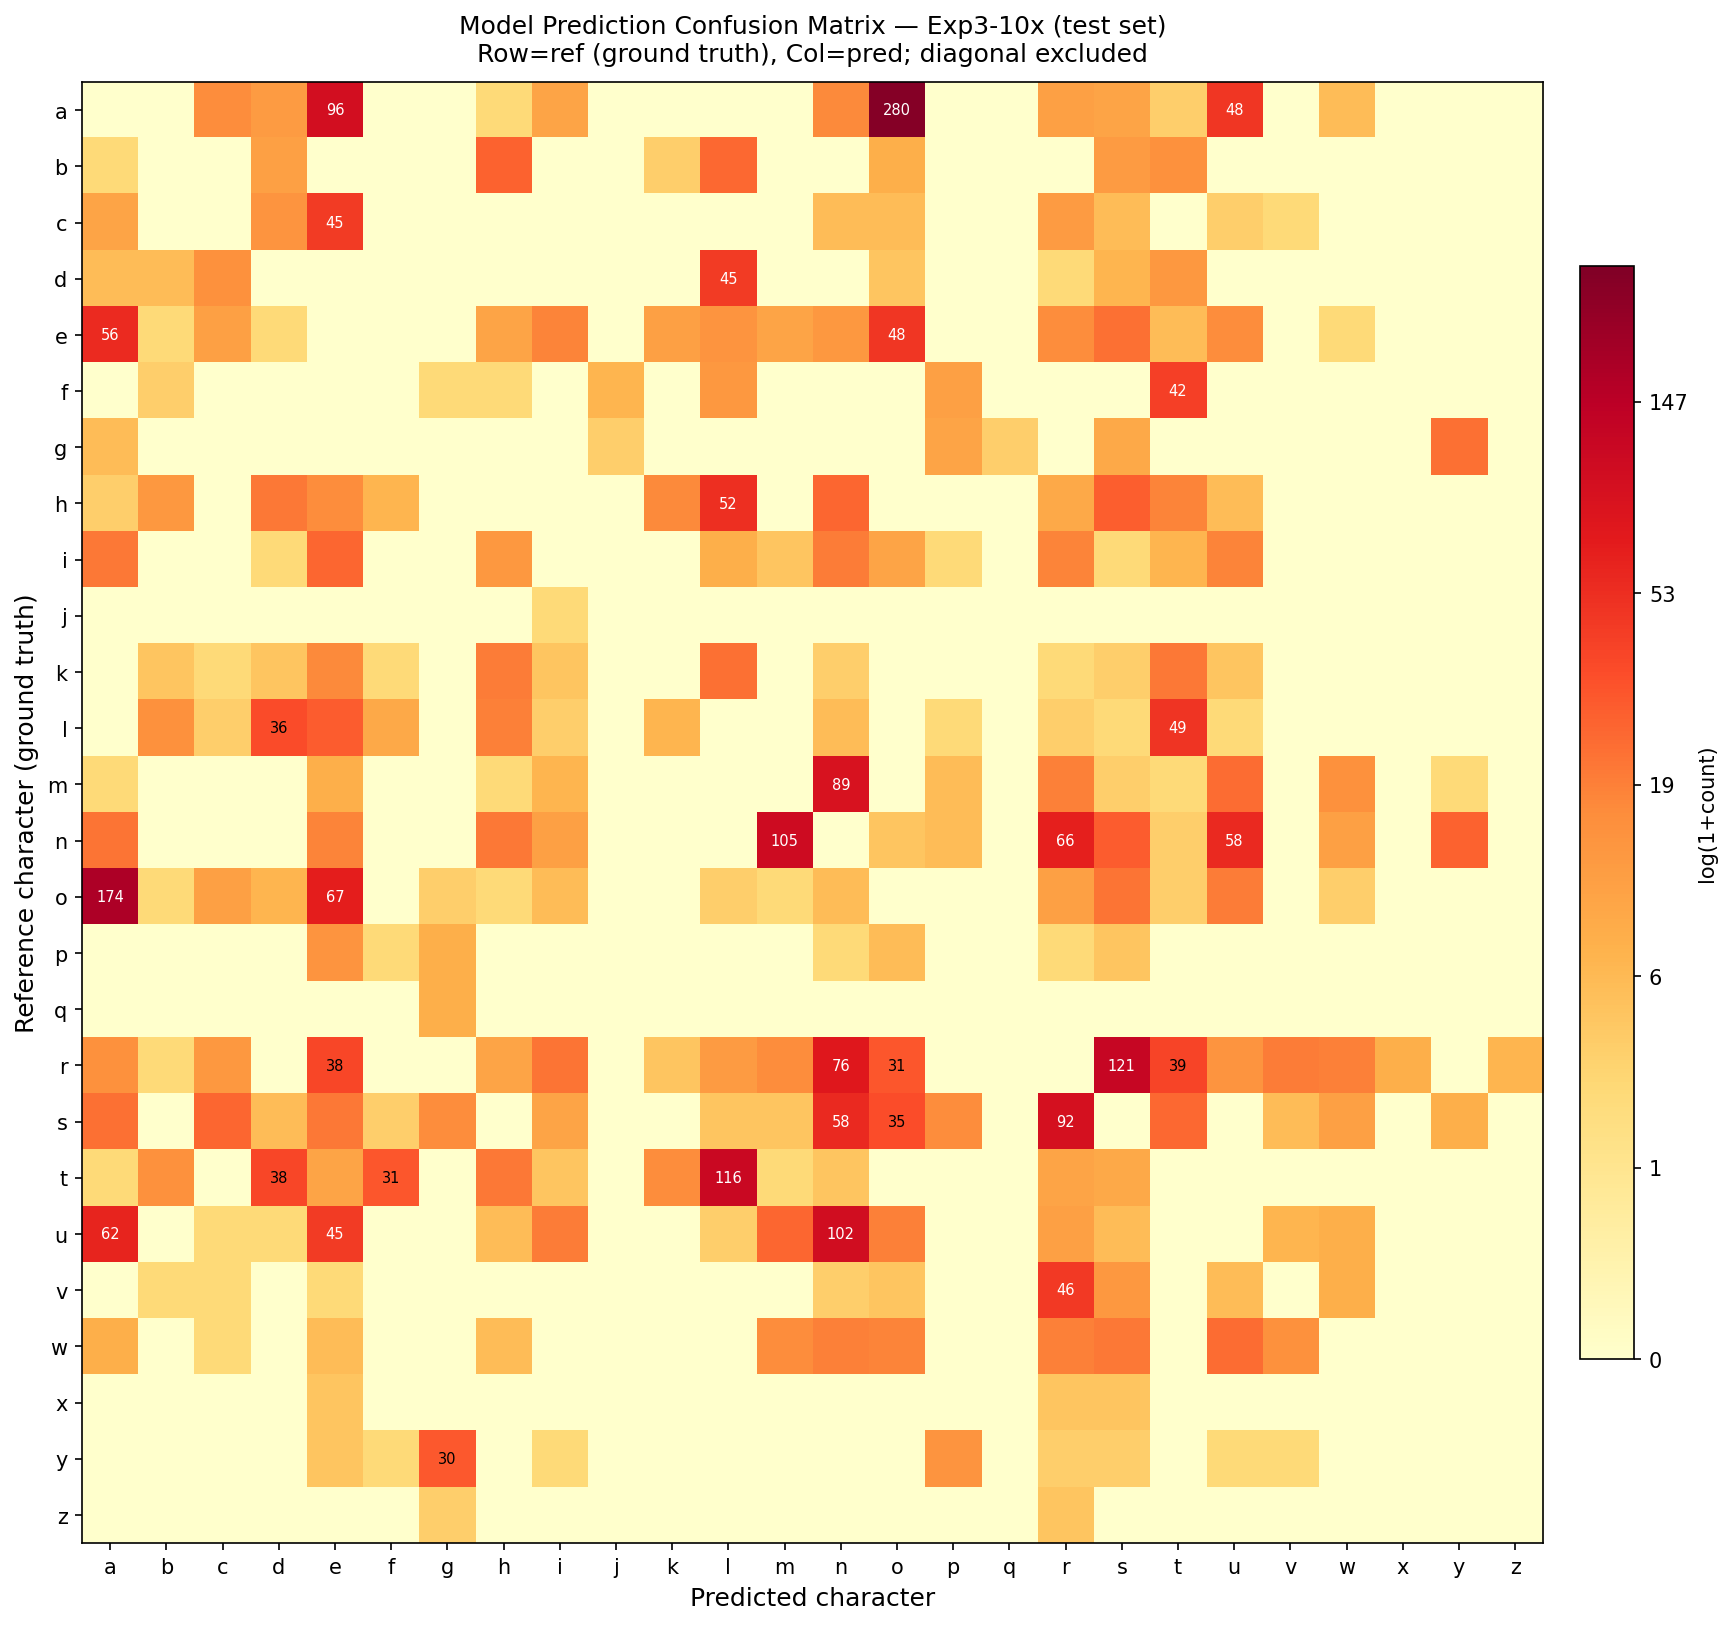
\includegraphics[width=\columnwidth]{model_confusion_matrix_exp3.png}
  \caption{Model prediction confusion matrix (Exp3-10x, full IAM + 10$\times$ synthetic). Row=ground truth, Col=predicted. Same $\log(1{+}\text{count})$ scale as Fig.~\ref{fig:vlmmatrix}. Top errors: \texttt{a}$\to$\texttt{o} (280), \texttt{o}$\to$\texttt{a} (174), \texttt{r}$\to$\texttt{s} (121).}
  \label{fig:modelmatrix_exp3}
\end{figure}

\begin{figure}[t]
  \centering
  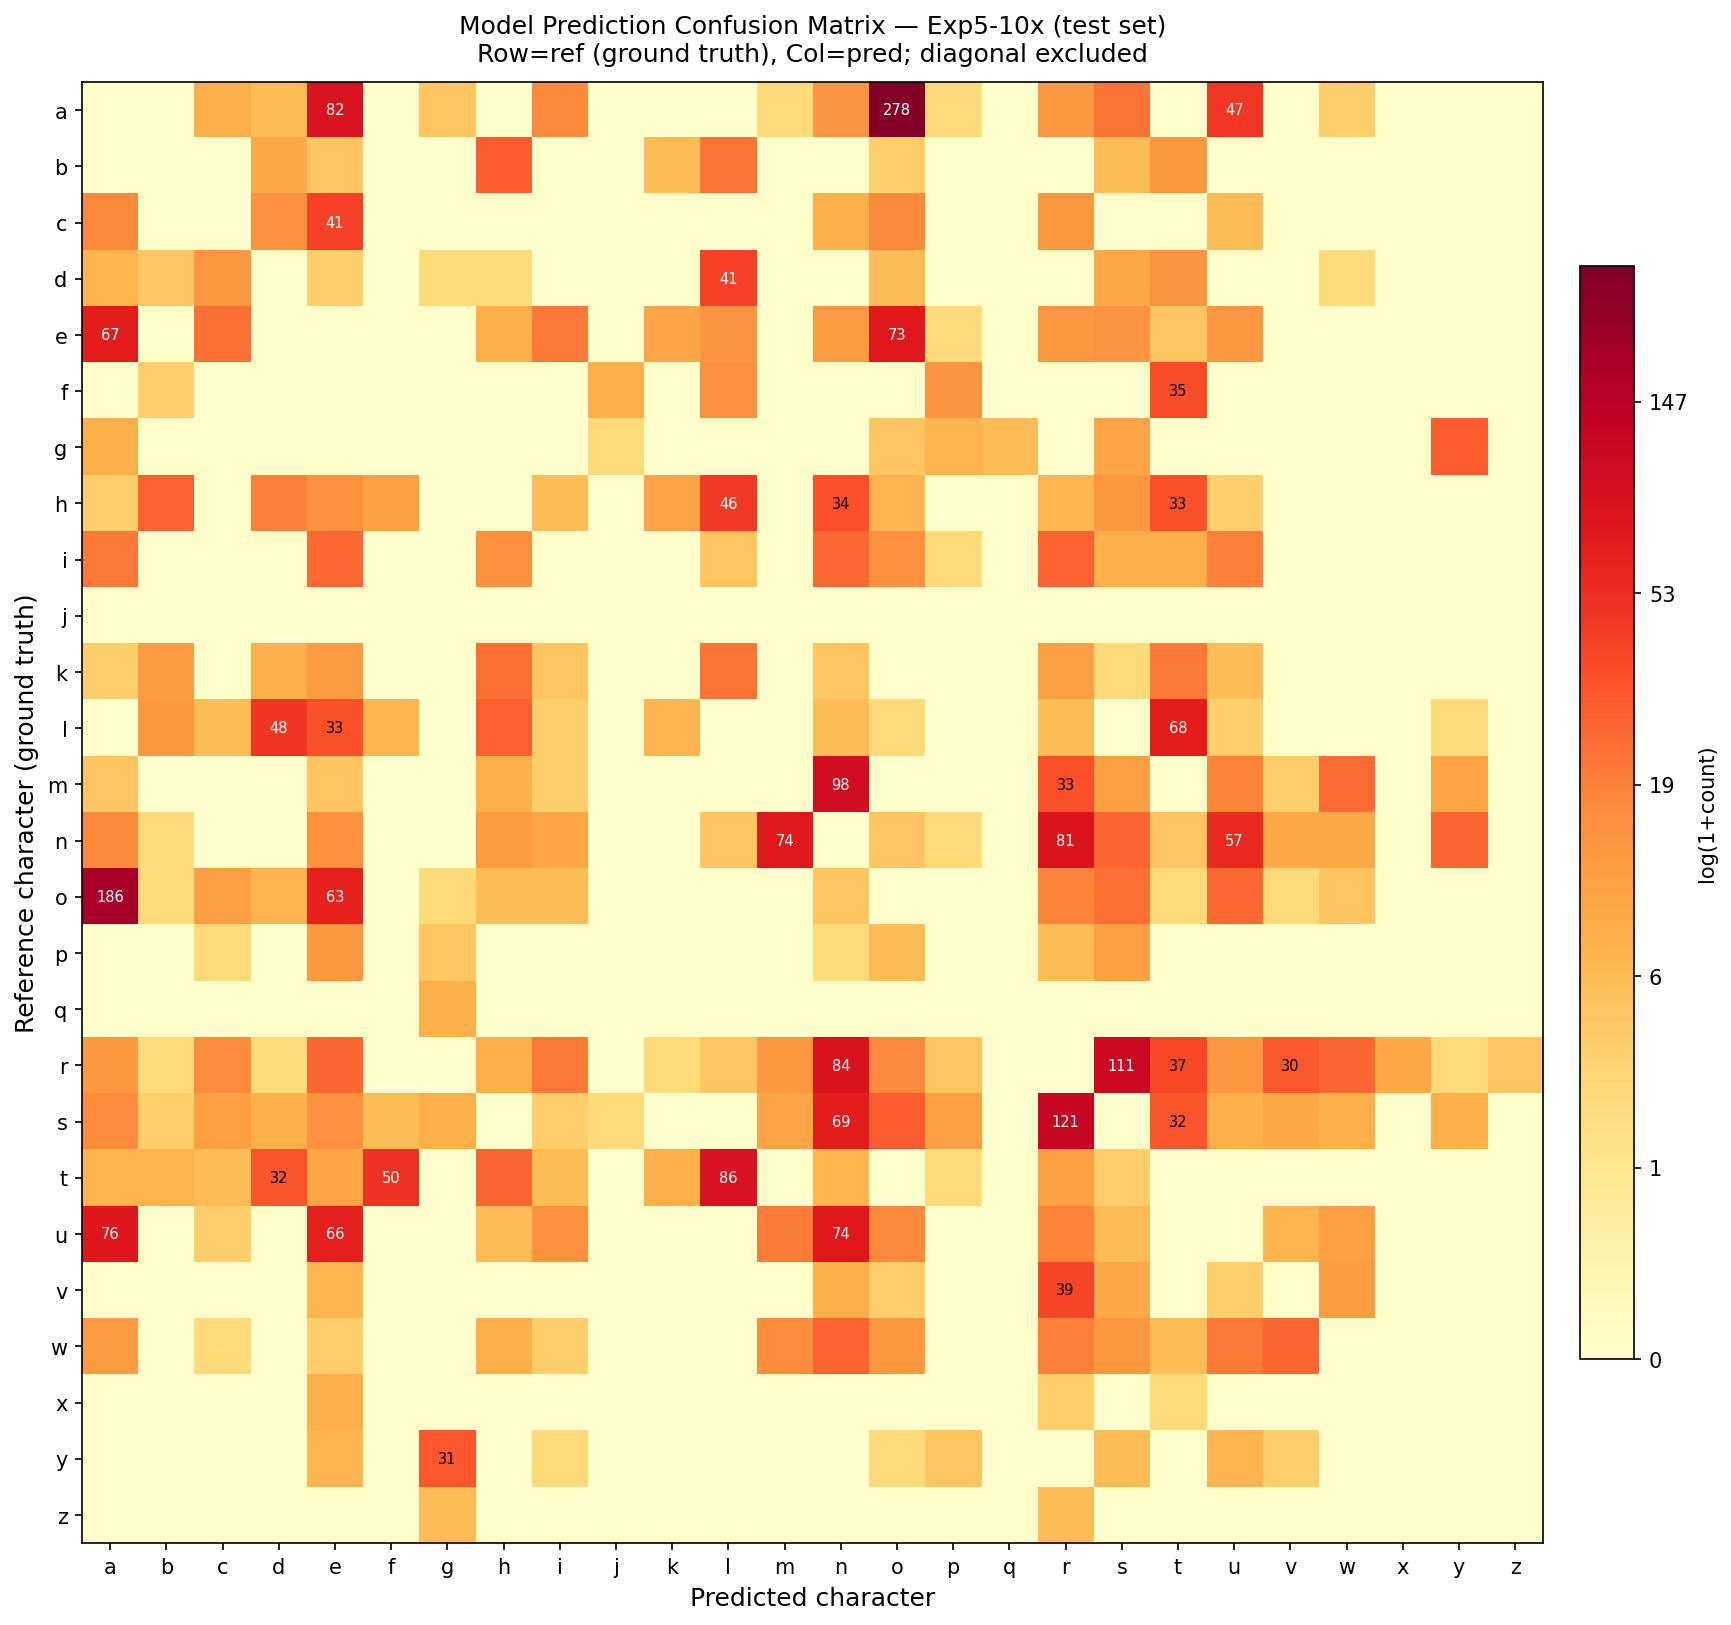
\includegraphics[width=\columnwidth]{model_confusion_matrix_exp5.png}
  \caption{Model prediction confusion matrix (Exp5-10x, V2-cleaned + 10$\times$ synthetic). Qualitatively identical to Fig.~\ref{fig:modelmatrix_exp3}: annotation cleaning changes overall CER but not \emph{which} pairs are hard.}
  \label{fig:modelmatrix_exp5}
\end{figure}

Figures~\ref{fig:vlmmatrix}--\ref{fig:modelmatrix_exp5} show the three heatmaps on a shared log-scale colormap. Both VLM and model concentrate errors on the \texttt{o}/\texttt{a}/\texttt{e} cluster and the \texttt{n}/\texttt{m}/\texttt{r}/\texttt{s} cluster. The model's raw counts are $2$--$3\times$ higher than the VLM's (max 280 vs.\ 99), reflecting cumulative errors over 2,915 test lines. Exp3 and Exp5 produce virtually identical patterns, confirming that annotation cleaning does not shift \emph{which} pairs are hard.

The $\rho=0.942$ for round/oval pairs is the strongest educational signal: a teacher configuring a system for penmanship feedback can draw directly on VLM confusion statistics to identify the character pairs most worth enforcing. The weaker $\rho=0.354$ for cross-category pairs indicates that beyond these visually motivated groups, the VLM and the model are driven by different error sources, motivating the OOV-gated design of our corrector.

%% ============================================================
\section{Configurable Decoding Pipeline}
%% ============================================================

\subsection{KenLM 4-gram Language Model}

We train a word 4-gram KenLM model~\cite{heafield2011} with modified Kneser-Ney smoothing on 183,468 sentences: IAM train+val labels ($\sim$7,400) and 176,010 lines from 20 Project Gutenberg novels. The model is 150MB (ARPA format). Beam search uses pyctcdecode with a 73,540-word mixed-case vocabulary. Initial vocabulary ablation shows that preserving original case is critical: lowercase-only vocab causes proper nouns to be penalized as unknown tokens (6.64\%$\to$6.41\% with mixed case).

\subsection{Full Three-Level Pipeline Results}

\begin{table}[h]
\centering
\caption{Three-Level Decoding Pipeline: Greedy $\to$ Beam+KenLM $\to$ Confusion Spell Correction (beam=50, $\alpha$=0.5, $\beta$=1.0, mixed-case vocab). Vocabulary ablation rows show beam-only results. Bold rows indicate best spell CER per series.}
\label{tab:beam}
\begin{tabular}{@{}llcccc@{}}
\toprule
\textbf{Exp} & \textbf{Scale} & \textbf{Greedy} & \textbf{Beam} & \textbf{Spell} & $\boldsymbol{\Delta_{\text{total}}}$ \\
\midrule
\multicolumn{6}{@{}l}{\textit{Vocabulary ablation (Exp3-10x, beam+4g)}} \\
Exp3-10x & unigram only   & 7.53\% & 7.50\% & ---    & $-$0.03\% \\
Exp3-10x & 4g (lowercase) & 7.53\% & 6.64\% & ---    & $-$0.89\% \\
Exp3-10x & 4g (mixed case)& 7.53\% & 6.41\% & ---    & $-$1.12\% \\
\midrule
\multicolumn{6}{@{}l}{\textit{Exp1/2 --- Baselines (no synthetic)}} \\
Exp1      & 0$\times$  & 8.48\% & 6.92\% & 6.74\% & $-$1.74\% \\
Exp2      & 0$\times$  & 10.38\%& 8.33\% & 8.15\% & $-$2.23\% \\
\midrule
\multicolumn{6}{@{}l}{\textit{Exp3 --- Full IAM + synthetic}} \\
Exp3-1x  & 1$\times$  & 7.92\% & 6.30\% & 6.10\% & $-$1.81\% \\
Exp3-2x  & 2$\times$  & 7.88\% & 6.45\% & 6.23\% & $-$1.64\% \\
Exp3-3x  & 3$\times$  & 7.67\% & 6.34\% & 6.13\% & $-$1.54\% \\
Exp3-5x  & 5$\times$  & 7.65\% & 6.27\% & 6.06\% & $-$1.58\% \\
Exp3-7x  & 7$\times$  & 7.75\% & 6.37\% & 6.15\% & $-$1.60\% \\
\textbf{Exp3-10x} & \textbf{10}$\boldsymbol{\times}$ & \textbf{7.53\%} & \textbf{6.20\%} & \textbf{5.94\%} & \textbf{$-$1.59\%} \\
\midrule
\multicolumn{6}{@{}l}{\textit{Exp4 --- V1-cleaned IAM + synthetic}} \\
Exp4-1x  & 1$\times$  & 8.96\% & 7.34\% & 7.10\% & $-$1.86\% \\
Exp4-2x  & 2$\times$  & 8.76\% & 7.19\% & 6.98\% & $-$1.77\% \\
\textbf{Exp4-3x}  & \textbf{3}$\boldsymbol{\times}$  & \textbf{8.61\%} & \textbf{7.09\%} & \textbf{6.91\%} & \textbf{$-$1.70\%} \\
Exp4-5x  & 5$\times$  & 8.88\% & 7.32\% & 7.09\% & $-$1.79\% $\uparrow$ \\
Exp4-7x  & 7$\times$  & 8.92\% & 7.32\% & 7.10\% & $-$1.82\% $\uparrow$ \\
Exp4-10x & 10$\times$ & 9.08\% & 7.48\% & 7.26\% & $-$1.82\% $\uparrow$ \\
\midrule
\multicolumn{6}{@{}l}{\textit{Exp5 --- V2-cleaned IAM + synthetic}} \\
Exp5-base & 0$\times$  & 8.38\% & 6.65\% & 6.43\% & $-$1.95\% \\
Exp5-1x  & 1$\times$  & 8.09\% & 6.58\% & 6.32\% & $-$1.78\% \\
Exp5-2x  & 2$\times$  & 7.99\% & 6.63\% & 6.45\% & $-$1.54\% \\
Exp5-3x  & 3$\times$  & 8.03\% & 6.57\% & 6.37\% & $-$1.66\% \\
\textbf{Exp5-5x}  & \textbf{5}$\boldsymbol{\times}$  & \textbf{7.92\%} & \textbf{6.46\%} & \textbf{6.29\%} & \textbf{$-$1.63\%} \\
Exp5-7x  & 7$\times$  & 8.17\% & 6.59\% & 6.39\% & $-$1.78\% \\
Exp5-10x & 10$\times$ & 8.06\% & 6.64\% & 6.47\% & $-$1.59\% \\
\bottomrule
\end{tabular}
\end{table}

\subsection{Confusion-Guided Spell Corrector and Configurable Tolerance}
\label{sec:corrector}

After beam decoding, we apply a word-level confusion spell corrector. The corrector operates as follows: for each decoded word that is out-of-vocabulary (OOV), it attempts single-character substitutions drawn from the model's confusion matrix. If any substitution produces an in-vocabulary word, the highest-confidence substitution is accepted. Only OOV tokens are corrected, preventing over-correction on already-valid words.

The confusion matrix is thresholded at $\tau$: only pairs with count $\geq \tau$ become correction rules. This threshold is the \textbf{teacher-configurable parameter}:

\begin{table}[h]
\centering
\caption{Configurable Confusion Tolerance (Exp3-10x model). $\tau$ controls the number of active correction rules and the trade-off between strict penmanship enforcement and content-focused grading. CER values span from beam-only to full-spell endpoints.}
\label{tab:tolerance}
\begin{tabular}{@{}clcl@{}}
\toprule
$\boldsymbol{\tau}$ & \textbf{Active Rules} & \textbf{Spell CER} & \textbf{Pedagogical Use} \\
\midrule
$\infty$ (off) & 0   & 6.20\% & No confusion correction \\
50             & 56  & $\sim$6.10\% & Lenient: content-focused grading \\
20             & 130 & $\sim$6.03\% & Balanced: general homework \\
\textbf{5}     & \textbf{300} & \textbf{5.94\%} & Strict: penmanship assessment \\
\bottomrule
\end{tabular}
\end{table}

The confusion rule table is stored as a human-readable CSV (e.g., \texttt{o,a,280}). Teachers can inspect, edit, or augment rules directly---for example, adding pairs specific to a student's known writing habits, or removing pairs involving characters not covered in a given lesson. This \emph{teacher-in-the-loop} design is a key distinguishing feature from end-to-end neural graders.

The three-level pipeline for our best configurations:
\begin{equation}
  \text{CER}_{\text{Exp3}}: 7.53\% \xrightarrow{\text{beam}} 6.20\% \xrightarrow{\text{spell}} 5.94\%
\end{equation}
\begin{equation}
  \text{CER}_{\text{Exp5}}: 7.92\% \xrightarrow{\text{beam}} 6.46\% \xrightarrow{\text{spell}} 6.29\%
\end{equation}

Spell correction adds $-$0.26\% for Exp3 and $-$0.17\% for Exp5. The smaller gain for Exp5 reflects a higher proportion of beam outputs already in-vocabulary (V2-cleaned training data produces cleaner predictions on common words). Exp5 peaks at $5\times$ rather than $10\times$ scale, consistent with its anchor-limited augmentation behavior.

A practical observation for educational deployment: \textbf{Exp3-1x + beam + spell (6.10\%)} is within 0.16\% of \textbf{Exp3-10x + beam + spell (5.94\%)}, despite 1/10th the synthetic data. This suggests that for schools with limited compute, $1\times$ synthetic augmentation plus the full decoding pipeline delivers near-optimal performance---the language model and spell corrector are more cost-effective than scaling synthetic volume.

%% ============================================================
\section{Discussion}
%% ============================================================

\subsection{Why VLM Cleaning Fails---and What to Do Instead}

The cross-matrix correlation ($\rho=0.636$, round/oval $\rho=0.942$) directly explains the V1 cleaning failure: both the VLM and the trained model find round/oval character pairs (\texttt{o}/\texttt{a}/\texttt{e}) genuinely ambiguous because they are ambiguous---the physical ink strokes are sometimes indistinguishable. A VLM flagging these as ``annotation errors'' and a model predicting the wrong character are both responding to the same stimulus. Removing VLM-flagged samples therefore removes the hardest, most informative training examples rather than label noise.

The practical implication: VLM-assisted data cleaning should be applied \emph{conservatively} with explicit false-positive suppression (V2 prompt design), and the resulting confusion patterns should be redirected into the post-processing stage rather than discarded. This is precisely the V2 + configurable corrector design we propose.

\subsection{The Anchor Effect: A Constraint for Educational Deployment}

The Exp4 results reveal a minimum real-data threshold for synthetic augmentation: below $\sim$5,000 annotated real samples, increasing synthetic scale \emph{increases} CER beyond $3\times$ (8.61\%$\to$9.07\% at $10\times$). For schools considering automated grading, this implies that a minimum annotated dataset of $\sim$5,000 student handwriting samples is needed before synthetic augmentation provides reliable benefit. Below this threshold, the model overfits to the font rendering domain.

\subsection{Cost-Efficiency Analysis for Practical Deployment}

\begin{table}[h]
\centering
\caption{Cost-Benefit Comparison (relative to Exp1 greedy baseline, 8.48\%)}
\label{tab:costbenefit}
\begin{tabular}{@{}lcc@{}}
\toprule
\textbf{Intervention} & \textbf{CER Gain} & \textbf{Deployment Cost} \\
\midrule
$10\times$ synthetic augmentation  & 0.95\% & High (GPU training)  \\
4-gram KenLM beam search           & 1.33\% & Low (inference only) \\
Confusion spell correction ($\tau=5$) & 0.26\% & Minimal (lookup table) \\
\midrule
\textbf{Full pipeline (beam+spell)} & \textbf{1.59\%} & \textbf{Low} \\
\bottomrule
\end{tabular}
\end{table}

KenLM beam search outperforms $10\times$ synthetic augmentation in absolute CER gain while requiring no model retraining---a compelling argument for inference-time investment over training-time investment in resource-constrained schools. The spell corrector adds a further 0.26\% gain at essentially zero marginal cost once the confusion table is computed.

\subsection{Limitations}

Our best result (5.94\%) remains approximately 3.05\% above TrOCR-Large (2.89\%). All experiments use IAM English handwriting; generalizability to other scripts, student age groups, or writing instruments is not demonstrated. Font-rendered synthetic data lacks stroke-level variability; diffusion-based handwriting synthesis would likely yield larger augmentation gains. The configurable corrector operates at the word level and cannot currently exploit sentence-level context for correction decisions.

%% ============================================================
\section{Conclusion}
%% ============================================================

We have presented a configurable handwriting recognition pipeline designed for educational assessment, where the tension between penmanship strictness and content-focused grading is resolved by a teacher-adjustable confusion threshold. The pipeline (CRNN-CTC $\to$ KenLM beam search $\to$ confusion spell corrector) achieves \textbf{5.94\% test CER} on IAM at its strictest setting, with the threshold continuously adjustable to lenient mode without retraining.

A cross-matrix correlation analysis ($\rho=0.636$ globally, $\rho=0.942$ for round/oval characters) shows that VLM annotation confusion and model prediction confusion reflect the same underlying visual ambiguity in cursive strokes. This validates VLM-derived confusion tables as cold-start priors for the configurable corrector---enabling meaningful deployment before student-specific training data is available---and explains why VLM annotation cleaning is prompt-sensitive: aggressive cleaning removes ambiguous-but-informative training examples.

Additional findings with practical implications: (1) a ``anchor effect'' sets a minimum real-data threshold ($\sim$5,000 samples) below which synthetic augmentation is counter-productive; (2) KenLM beam search provides greater CER reduction (1.33\%) than $10\times$ synthetic augmentation (0.95\%) at lower deployment cost; (3) $1\times$ synthetic augmentation with the full decoding pipeline (6.10\% CER) is within 0.16\% of $10\times$ augmentation (5.94\%), supporting cost-effective deployment.

\textbf{Future work:} (1) User studies with teachers to validate the configurable threshold against real grading decisions; (2) Extension to student-specific confusion adaptation (personalized confusion tables per student); (3) Integration of model prediction confidence for uncertainty-aware grading feedback; (4) Diffusion-based handwriting synthesis for higher-quality augmentation; (5) Evaluation on multilingual educational handwriting datasets.

%% ============================================================
\bibliographystyle{IEEEtran}
\begin{thebibliography}{99}

\bibitem{shi2016}
B.~Shi, X.~Bai, and C.~Yao, ``An end-to-end trainable neural network for image-based sequence recognition,'' \textit{IEEE Trans.\ Pattern Anal.\ Mach.\ Intell.}, vol.~39, no.~11, pp.~2298--2304, 2016.

\bibitem{graves2006}
A.~Graves, S.~Fern\'andez, F.~Gomez, and J.~Schmidhuber, ``Connectionist temporal classification: Labelling unsegmented sequence data with recurrent neural networks,'' in \textit{Proc.\ ICML}, 2006.

\bibitem{li2021}
M.~Li et al., ``TrOCR: Transformer-based optical character recognition with pre-trained models,'' \textit{arXiv:2109.10282}, 2021.

\bibitem{retsinas2022}
G.~Retsinas, P.~Sfikas, B.~Gatos, and C.~Nikou, ``Best practices for a handwritten text recognition system,'' \textit{arXiv:2404.11339}, 2022.

\bibitem{marti2002}
U.-V.~Marti and H.~Bunke, ``The IAM-database: An English sentence database for offline handwriting recognition,'' \textit{Int.\ J.\ Document Anal.\ Recognit.}, vol.~5, no.~1, pp.~39--46, 2002.

\bibitem{frenay2014}
B.~Fr\'enay and M.~Verleysen, ``Classification in the presence of label noise: A survey,'' \textit{IEEE Trans.\ Neural Netw.\ Learn.\ Syst.}, vol.~25, no.~5, pp.~845--869, 2014.

\bibitem{jiang2025}
X.~Jiang et al., ``When VLMs meet image classification: Test sets renovation via VLM-guided generative data augmentation,'' \textit{arXiv:2505.16149}, 2025.

\bibitem{belval2019}
E.~Belval, ``TextRecognitionDataGenerator,'' GitHub, 2019. [Online]. Available: \url{https://github.com/Belval/TextRecognitionDataGenerator}

\bibitem{luo2023}
C.~Luo, L.~Jin, and Z.~Sun, ``CNN-BiLSTM model for English handwriting recognition,'' \textit{arXiv:2307.00664}, 2023.

\bibitem{hannun2014}
A.~Hannun et al., ``Deep Speech: Scaling up end-to-end speech recognition,'' \textit{arXiv:1412.5567}, 2014.

\bibitem{heafield2011}
K.~Heafield, ``KenLM: Faster and smaller language model queries,'' in \textit{Proc.\ WMT}, 2011.

\bibitem{gao2023}
Y.~Gao et al., ``Automated grading of handwritten assignments using deep learning: Challenges and opportunities,'' in \textit{Proc.\ AIED}, 2023.

\bibitem{burrows2015}
S.~Burrows, I.~Gurevych, and B.~Stein, ``The eras and trends of automatic short answer grading,'' \textit{Int.\ J.\ Artif.\ Intell.\ Educ.}, vol.~25, no.~1, pp.~60--117, 2015.

\bibitem{wigington2017}
C.~Wigington et al., ``Data augmentation for recognition of handwritten words and lines using a CNN-LSTM network,'' in \textit{Proc.\ ICDAR}, 2017.

\end{thebibliography}

%% ============================================================
\appendix
\section{Hyperparameter Search Full Configuration}

\begin{table}[h]
\centering
\caption{All 14 Hyperparameter Search Configurations}
\label{tab:hparam_full}
\begin{tabular}{@{}ccccccc@{}}
\toprule
\textbf{Run} & \textbf{hid} & \textbf{drop} & \textbf{bs} & \textbf{lr} & \textbf{cnn} & \textbf{wd} \\
\midrule
00 & 256 & 0.1 & 64 & 1e-4 & 512 & 1e-4 \\
01 & 128 & 0.1 & 64 & 1e-4 & 512 & 1e-4 \\
02 & 512 & 0.1 & 64 & 1e-4 & 512 & 1e-4 \\
03 & 512 & 0.0 & 64 & 1e-4 & 512 & 1e-4 \\
04 & 512 & 0.2 & 64 & 1e-4 & 512 & 1e-4 \\
05 & 512 & 0.3 & 64 & 1e-4 & 512 & 1e-4 \\
06 & 512 & 0.1 & 32 & 1e-4 & 512 & 1e-4 \\
07 & 512 & 0.1 & 128 & 1e-4 & 512 & 1e-4 \\
08 & 512 & 0.1 & 64 & 3e-4 & 512 & 1e-4 \\
09 & 512 & 0.1 & 64 & 5e-5 & 512 & 1e-4 \\
10 & 512 & 0.1 & 64 & 1e-4 & 256 & 1e-4 \\
11 & 512 & 0.1 & 64 & 1e-4 & 512 & 1e-3 \\
12 & 512 & 0.1 & 64 & 1e-4 & 512 & 0.0 \\
13 & 512 & 0.1 & 64 & 1e-4 & 512 & 1e-4 \\
\bottomrule
\end{tabular}
\end{table}

\section{VLM Audit Prompt Comparison}

\textbf{V1 Prompt (aggressive, flag rate 33\%):}
\begin{quote}\small
\textit{The image shows a single line of handwritten English text. The claimed annotation is: ``\{annotation\}''. Compare word by word. Reply CORRECT / INCORRECT / AMBIGUOUS. Rules: INCORRECT: use whenever you can read a word and it differs. Err on the side of flagging. AMBIGUOUS: only when ink is too faded to read at all.}
\end{quote}

\textbf{V2 Prompt (conservative, flag rate 12.6\%):}
\begin{quote}\small
\textit{The image shows a single line of handwritten English text from the IAM Handwriting Database, annotated by trained human experts (expected $\sim$95\%+ accuracy). Annotation: ``\{annotation\}''. Default to CORRECT. Only flag INCORRECT when ALL of the following: you can clearly read the word; the difference is unambiguous; you can specify exactly which characters differ. Do NOT flag: digit 0 vs letter O (IAM uses 0 for zero; trust annotation), minor punctuation, British spelling, abbreviations, proper nouns, handwriting style variations.}
\end{quote}

\end{document}
